\documentclass{bigdata}
\usepackage[utf8]{inputenc}
\usepackage{tocloft}
\usepackage{multirow}

\renewcommand\cftsecfont{\small}
\renewcommand\cftsubsecfont{\small}

\DeclareMathOperator*{\argmax}{arg\,max}
\DeclareMathOperator*{\argmin}{arg\,min}

\title{Content-Based 3D Shape Retrieval System}
\author{Diego Renders (5740894) and Florian-Claudiu Gheorghică (6924123)}
\date{October 2019}
\onecolumn

\begin{document}
\setlength{\cftbeforesecskip}{1pt}
\maketitle

\newpage

\tableofcontents

\section{Introduction}

This is a technical report detailing the implementation of a content-based 3D shape retrieval system. The aim of this implementation is the exploration of existing techniques for shape querying using meaningful 3D descriptors, either scalar or histogram-based. To this effect, the Princeton Shape Database is used to evaluate the system in an environment closer to a real life application than if a smaller database would be used.

\subsection{Overview}
This introductory section concludes with a short overview of existing related work. The technologies used for the application are then listed and briefly described. The Pre-processing section explains the choices of dataset, granularity and vertex count before detailing the database creation and normalization pipeline. The Feature Extraction section lists and explains the features that are implemented in our system, as well as some reasoning behind the design of the feature vector. The Matching section explains our distance function and how shape matching is actually performed using a kd-tree and k-nearest neighbors. Before evaluation, a t-SNE-powered visualization of the feature space of our database is provided. After this, the database is evaluated using MAP and precision at k and some query examples are given. Finally, the conclusions sum up our system's behavior and explore the limitations within our project, as well as the possibilities for improvement and future work.

\subsection{System Specifications}
All testing has been performed on a Dell Inspiron 7577 with a Windows 10 Pro 64-bit operating system, 16 GB of RAM, an Intel(R) Core(TM) i7-7700HQ CPU @ 2.80 GHz (8CPUs) and NVIDIA Geforce GTX 1060 with Max-Q Design video card.

\subsection{Motivation}
This project was created as part of the \textit{Multimedia Retrieval} course held by Prof. Dr. Alexandru Telea at the University of Utrecht.

\subsection{Literature review}
Vranić \& Saupe (2003), Körtgen et al. (2003) and Tangelder \& Veltkamp (2007) provide a thorough overview of classical 3D shape retrieval methods using shape descriptors. The features used in this project are also explained in their work. Surveying the existing methods, Tangelder \& Veltkamp generated a diagram showing the conceptual framework for shape retrieval applications (\textit{Figure 1}). This diagram also describes how our application is structured on a high level, minus any implied online functionality.

\begin{figure}[h!]
	\centering
	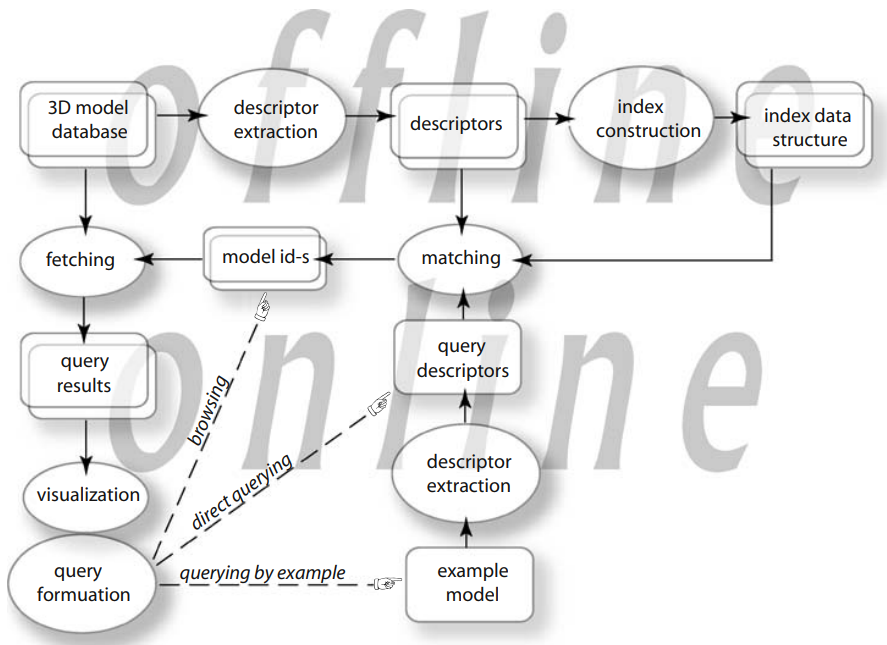
\includegraphics[width=0.7\linewidth]{Pictures/conceptualdiagram.png}
	\caption{Tangelder \& Veltkamp (2007), Conceptual framework for shape retrieval.}
\end{figure}
 
\noindent Feng et al. (2016) use a different approach than the one described in this paper, using voxel shapes and skeleton descriptors for shape matching. Even so, some alternative Histogram matching techniques are presented, including Earth Mover's Distance and Multilevel Distance, which could represent viable alternatives to the histogram distance function used in our implementation.

\noindent Song (2017) describes some advanced indexing techniques for multimedia data retrieval which we make use of in our project in order to speed up searching. Most notably, he provides some details of kd-tree functionality, as well as some alternative approaches to dimensionality reduction.

\section{Technologies Used}
This section will list the external libraries used in developing the application. The two programming languages used are C++ for the shape retrieval system and Python for plots and visualization. C++ was selected for its speed and Python for its ease of use.
\subsection{C++}
\paragraph{ALGLIB v3.15.0 Free Edition}
ALGLIB is a cross-platform numerical analysis and data processing library. It contains tools for data analysis, optimization and nonlinear solvers, interpolation and linear/non-linear least-squares fitting, linear algebra and many other algorithms. In our implementation, it is used for PCA. Details can be found here: https://www.alglib.net/.
\paragraph{ANN v1.1.2}
ANN (A Library For Approximate Nearest Neighbor Searching) is a library written in C++, which supports data structures and algorithms for both exact and approximate nearest neighbor searching in arbitrarily high dimensions. This is used in our implementation to speed up shape matching using k-nearest neighbors. More details can be found here: https://www.cs.umd.edu/~mount/ANN/.
\paragraph{nupengl.core}
This NuGet package contains various libraries required to build OpenGL applications, including FreeGLUT, GLFW and GLEW. Details can be found here: https://www.nuget.org/packages/nupengl.core/.
\paragraph{PMP Library v1.1.0}
The Polygon Mesh Processing (PMP) library contains three main modules used for mesh processing: core (used for data representation), algorithm (used for algorithm implementations) and visualization (used for OpenGL-based visualization). Out of these, the algorithm module is used in our system for mesh decimation. More information, as well as a download link, can be found at: https://www.pmp-library.org/.
\paragraph{3D Unstructured Grid Implementation}
The application uses a 3D unstructured grid implementation provided by the University of Groningen as part of their Data Visualization Book. Basic visualization using OpenGL as well as a PLY file reader are also included. The implementation can be found here: http://www.cs.rug.nl/svcg/uploads/DataVisualizationBook/sp3\_grids.zip
\paragraph{ZPR v0.4}
Zoom, Pan and Rotate (ZPR) is a mouse manipulation module for C or C++ GLUT/OpenGL programs. In our project, ZPR enables mouse zooming, panning and rotation when visualizing a 3D shape. The implementation may be found here: http://www.nigels.com/glt/gltzpr/.

\subsection{Python}
\paragraph{matplotlib v3.1.1}
Matplotlib is a Python 2D plotting library. It is a requirement for the Seaborn library which was used for generating the 2D plot of the t-SNE result. Website: https://matplotlib.org/.
\paragraph{numpy}
Numpy is a fundamental package for scientific computing with Python, as it contains a powerful N-dimensional array object used by other scientific python libraries, such as pandas. Details can be found here: https://numpy.org/.
\paragraph{pandas v0.25.3}
Pandas in an open source library providing high-performance, easy-to-use data structures and data analysis tools for Python. The data frame structure it contains can be used with seaborn to simplify plotting. Website: https://pandas.pydata.org/.
\paragraph{seaborn v0.9.0}
Seaborn is a Python data visualization library based on matplotlib. It provides a high-level interface for drawing graphs. Seaborn was used to draw the scatter plot resulting from our t-SNE implementation. Details about the library can be found here: https://seaborn.pydata.org/.
\paragraph{t-SNE Implementation}
T-Distributed Stochastic Neighbor Embedding (t-SNE) is a technique for dimensionality reduction that is well suited for high-dimensional dataset visualization. Our project uses the implementation by Laurens van der Maaten for the Python language, which can be downloaded here: https://lvdmaaten.github.io/tsne/code/tsne\_python.zip. More details about t-SNE can be found on the official web page: https://lvdmaaten.github.io/tsne/.

\section{Pre-processing}

\subsection{Database selection}
For the purpose of this project, the Princeton Shape Benchmark (PSB) database of 3D models was selected. Details about this set of 3D models can be found in (Shilane, P. et al, 2004) or on the official website: https://shape.cs.princeton.edu/benchmark/. \\
This dataset was chosen due to its size, variety, cleanliness and its good options of granularity in terms of classes. A bigger, more diverse database will more accurately reflect the more difficult real-world applications. In addition, the chosen granularity of 53 leaf classes permits for mostly homogeneous shapes within the same class, e.g. the winged vehicle class, while also a flying object, should be very different from the balloon class. Conversely, any coarser the granularity would mean too many classes that would be too specific, which would interfere with the evaluation step. 

\subsection{File reading}

The files from the PSB were all provided in the OFF file format and an OFF reader was initially considered as a starting point. However, as a PLY format reader was likely to be necessary in the long-term, an OFF-to-PLY converter was written in order to enforce PLY as the default format for the application.
This converter simply creates a PLY header using data from the OFF file, then copies the vertex and face data over. While not a scalable approach for more complex OFF files, the converter was able to successfully process the entire PSB database.

\subsection{Database evaluation}
The database contains 1814 models in the OFF file format. All of the models contain only triangles as faces. The distribution of faces is shown in figure 1. The average number of vertices is 4221, the minimum 10, and the maximum 160940. The histogram, along with the average, shows that most of the models have a vertex count of smaller than twenty thousand. In order to successfully perform the upcoming steps of feature extraction the models need to have approximately the same number of vertices. Two actions can be undertaken to achieve this, supersampling and subsampling. Supersample the models with a low vertex count, and subsample the models with a large vertex count. A target number of vertices has to be chosen for this. One solution could be to choose the average. However because several of the meshes have a very high resolution (a hundred thousand vertices), subsampling this to reach the four thousand required vertices would ruin the original shape. Therefore the target vertices is chosen to be higher than the average, so that the higher resolution models retain their characteristics. The only downside for choosing a higher target number of vertices is an increase in computation time. The target number of vertices is set at twenty thousand, and the methodology for supersampling and subsampling is explained in the following two sections.

\begin{figure}[h!]
  \centering
    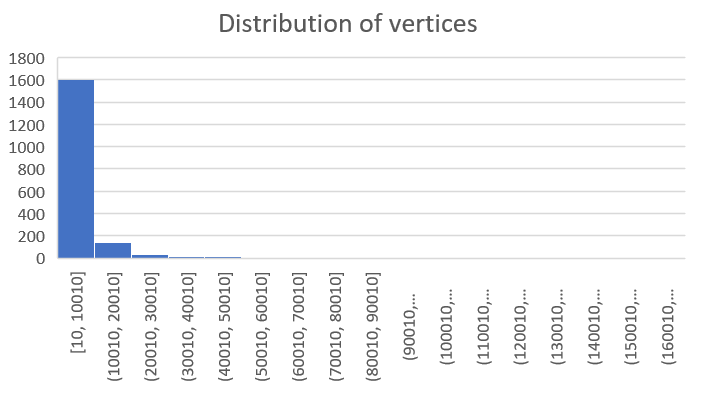
\includegraphics[width=0.7\linewidth]{Pictures/verticesHist.png}
    \caption{Histogram showing the distribution of vertices in the PSB database}
\end{figure}

\subsection{Supersampling}
Supersampling is done in this implementation by splitting a larger triangle into 4 smaller ones via adding the midpoints of the original triangle’s edges as vertices and using them to form new triangles with the original vertices. An example is shown below:

\begin{figure}[h!]
  \centering
  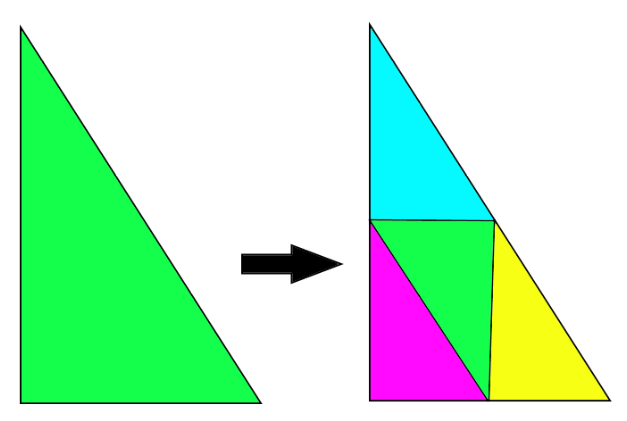
\includegraphics[width=0.5\linewidth]{Pictures/triangle.png}
  \caption{Supersampling Example}
\end{figure}


\noindent To ensure the triangles obtained like this are not outliers in terms of their size, the cells in the model were first sorted by their area inside a vector, from smallest to largest. The area of each cell was calculated using the following formula:

\begin{equation}
S = \frac{|AB||AC|sin(\theta)}{2}
\end{equation}\\

\noindent Thus, at each step, only the triangle with the largest surface is split up into smaller triangles. The original triangle is removed from the vector, and the smaller triangles are inserted at positions that do not disturb the ordered property of the data structure.

\subsection{Subsampling}
For the task of subsampling the Polygon Mesh Processing (pmp) library is used. The SurfaceSimplification class is used to perform mesh decimation, taking as input the mesh and a target number of vertices. To demonstrate that this algorithm works correctly for our models a pre and post visualisation is shown in figure 2. This is the largest model in the dataset with 316.498 faces and 160.940 vertices. The post decimation model contains 78.473 faces and 40.000 vertices in the middle picture and 20.000 vertices in the right picture. Even though the model only has a fourth of its original vertices in the second case, it clearly retains its characteristics. And even when the vertex count is brought down to 20.000 vertices it is hard to distinguish them. Therefore we can conclude that the algorithm is a suitable tool for this project.

\begin{figure}[h!]
  \centering
  \begin{subfigure}[b]{0.3\linewidth}
    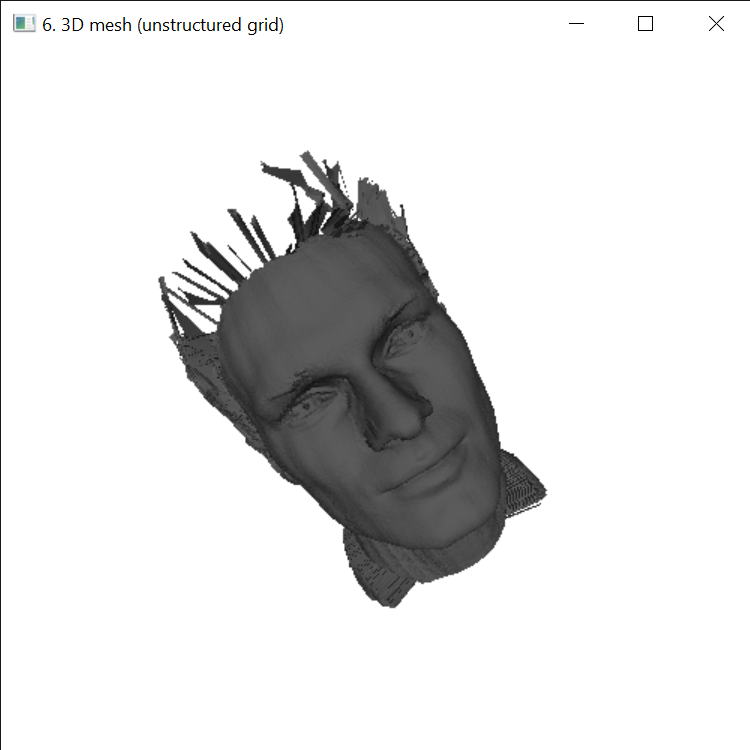
\includegraphics[width=\linewidth]{Pictures/preSub.png}
    \caption{160k vertices}
  \end{subfigure}
  \begin{subfigure}[b]{0.3\linewidth}
    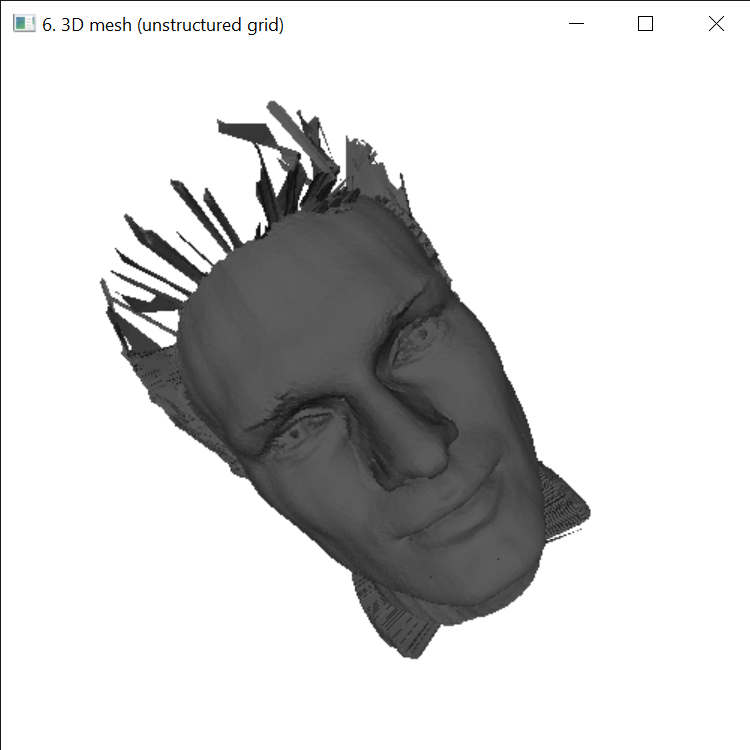
\includegraphics[width=\linewidth]{Pictures/postSub.png}
    \caption{40k vertices}
  \end{subfigure}
  \begin{subfigure}[b]{0.3\linewidth}
    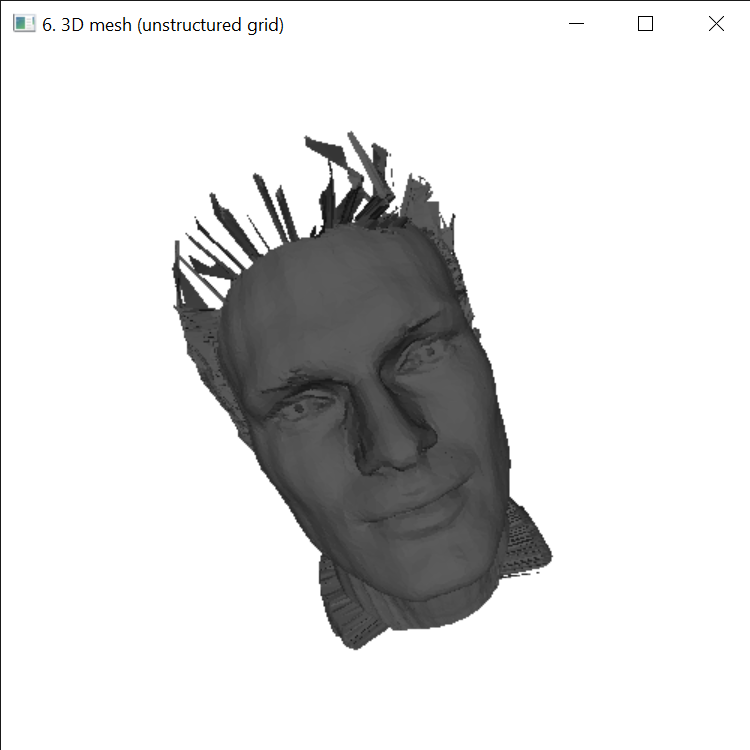
\includegraphics[width=\linewidth]{Pictures/postSub2.png}
    \caption{20k vertices}
  \end{subfigure}
  \caption{Results of mesh decimation for model m303}
  \label{fig:decimatedMesh}
\end{figure}

\subsection{Four step normalization}

Next each mesh will go through the four step normalization pipeline so that it is ready to be used in upcoming tasks. Figure 1 shows a visualization of what each step does, the red, green, and blue represent the $x$, $y$, and $z$ axises respectively from zero to one. The first step is to center on the Barycenter, than in step 2 PCA is done to orient the object in an intuitive way. Step 3 performs a fliptest which result in the majority of the mass in the object to be located in the negative side of the axis. Finally step 4 normalizes the model, which is excluded in the figure because the model was already normalized and thus would show no difference.

\begin{figure}[h!]
  \centering
  \begin{subfigure}[b]{0.4\linewidth}
    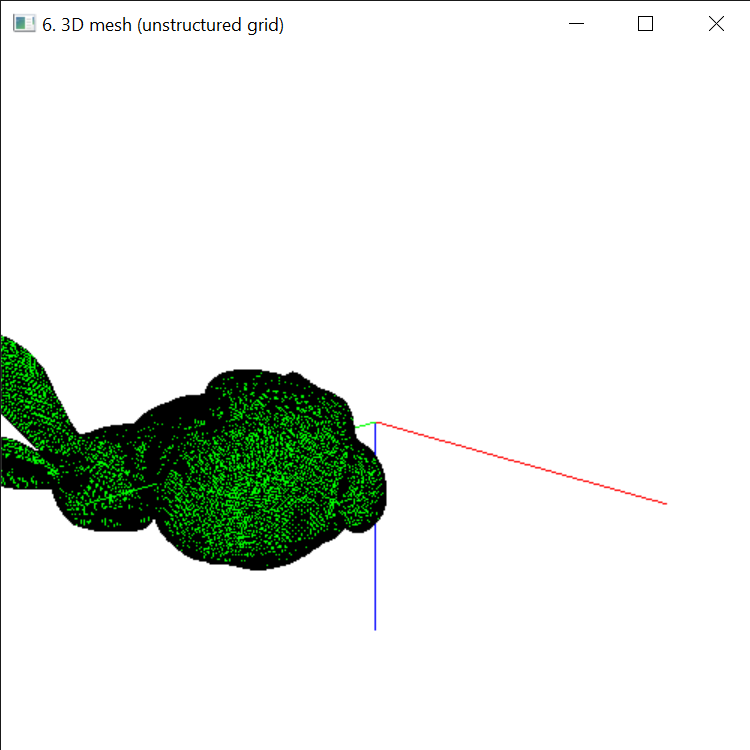
\includegraphics[width=\linewidth]{Pictures/Part2/Step0.png}
    \caption{Step 0}
  \end{subfigure}
  \begin{subfigure}[b]{0.4\linewidth}
    \includegraphics[width=\linewidth]{Pictures/Part2/step1.png}
    \caption{Step 1 Barycenter}
  \end{subfigure}
  \begin{subfigure}[b]{0.4\linewidth}
    \includegraphics[width=\linewidth]{Pictures/Part2/step2.png}
    \caption{Step 2 PCA}
  \end{subfigure}
  \begin{subfigure}[b]{0.4\linewidth}
    \includegraphics[width=\linewidth]{Pictures/Part2/step3.png}
    \caption{Step 3 Fliptest}
  \end{subfigure}
  \caption{Visualization of the Four step normalization pipeline.}
  \label{fig:bunny}
\end{figure}

\subsubsection{Center on the barycenter}

For the first step the barycenter $b$ is calculated, which is the average x, y, and z coordinates of all vertices in the mesh. Next, each vertex $v$ is translated, by subtracting these averages from each of its points resulting in the new vertex position $u$.
\[
\begin{bmatrix}
u_x \\
u_y \\
u_z \\
\end{bmatrix}
=
\begin{bmatrix}
v_x \\
v_y \\
v_z \\
\end{bmatrix}
-
\begin{bmatrix}
b_x \\
b_y \\
b_z \\
\end{bmatrix}
\]

The result can be verified by calculating the average coordinates again, which should be 0 after the normalization.

\subsubsection{PCA}
Principal component analysis is done using the alglib library. The three eigenvectors $e_1$, $e_2$, and $e_3$ are returned by the algorithm. These three vectors are orthogonal to each other. Therefore these eigenvectors can easily be made to coincide with the x, y, and z axis, because the model only has to be rotated. A rotation matrix M is than created using the vectors $x$, $y$, and $z$, that represent the axes of the normal coordinate system. The eigenvector corresponding to the largest eigenvalue will coincide with the x axis, the next eigenvector with the y axis, and the final one with the z axis.

\[
x = 
\begin{bmatrix}
1 \\
0 \\
0 \\
\end{bmatrix}
y =
\begin{bmatrix}
0 \\
1 \\
0 \\
\end{bmatrix}
z =
\begin{bmatrix}
0 \\
0 \\
1 \\
\end{bmatrix}
M =
\begin{bmatrix}
x \cdot e_1 & x \cdot e_2 & x \cdot e_3 \\
y \cdot e_1 & y \cdot e_2 & y \cdot e_3 \\
z \cdot e_1 & z \cdot e_2 & z \cdot e_3 \\
\end{bmatrix}
\]

The new vertex $u$ is obtained by multiplying this matrix with the old vertex $v$.

\[
\begin{bmatrix}
u_x \\
u_y \\
u_z \\
\end{bmatrix}
=
M
\cdot
\begin{bmatrix}
v_x \\
v_y \\
v_z \\
\end{bmatrix}
\]

The result of the translation can easily be verified. Doing PCA again on the translated mesh returns three eigenvectors that now correspond with the $x$, $y$, and $z$ axis.

\subsubsection{Fliptest}
The eigenvectors used for the translation in the previous step are unoriented and thus give no information about to which side the model should be directed. Using the fliptest it is ensured that the majority of the mass resides in the negative half-space. Mass in this case is not indicated by the number of the vertices but also takes momentum into consideration, i.e. vertices farther away from the origin have a higher weight. Three variables are introduced: $w_x$, $w_y$, and $w_z$ that indicate the total weight of each of three coordinates. 
\begin{equation}
w_i = \sum sign(C_{t,i})(C_{t,i})^2
\end{equation}
 where $C_{t,i}$ is the $i^{th}$ coordinate of triangle t ($i \in {x,y,z}$). The latter part of the summation gives coordinates far away from the origin an higher weight, while the former part gives it either a negative or positive weight. These values are than used for a new scaling matrix $M$. Which flips the coordinates if necessary, in case the mesh is already properly oriented $M$ will simply be the identity matrix.
\[
M = 
\begin{bmatrix}
sign(w_x) & 0 & 0 \\
0 & sign(w_y) & 0 \\
0 & 0 & sign(w_z) \\
\end{bmatrix}
\]

\subsubsection{Normalization}
The last step scales the model in the unit volume, i.e. it can fit in a unit cube. First the min and max of the $x$,$y$, and $z$ coordinates of the axis-aligned bounding box is found. Next the largest distance $\delta$ between the min and max of these coordinates is used for the scaling factor $s = \frac{1}{\delta}$. Finally each vertex $v$ is multiplied with this factor to obtain the new vertex $u$.

\[
\begin{bmatrix}
u_x \\
u_y \\
u_z \\
\end{bmatrix}
=
\begin{bmatrix}
v_x \\
v_y \\
v_z \\
\end{bmatrix}
\cdot s
\]

A visualization is excluded, however the effectiveness of this step can easily be verified by looking at the resulting bounding box of the model.

\subsection{Verifying the normalization}
Next for each model in the database the following steps are performed: 
1. if the model has less than 20.000 vertices use mesh decimation with target number of vertices set to 20.000.
2. if the model has mor than 20.000 vertices use supersampling with target number of vertices set to 20.000.
3. Center the model on its barycenter.
4. Perform PCA and use align the eigenvectors with the x, y, and z axis.
5. Flip the model if necessary.
6. Normalize in a unit cube.
In total 21 files were unable to processed, leaving a total of 1796 models in the new dataset. To verify that all the steps were performed correctly a new overview of the database can be created. The minimum number of vertices is 20.000, the maximum is 22963, the average is 200006, and standard deviation 116.61. These numbers show that the subsampling and supersampling worked correctly. There are a few models with a higher than average vertex count, because they were unable to processed by the $pmp$ mesh decimation algorithm. However they are still included in the final dataset because their vertex count is close enough to 20.000.

\section{Feature Extraction}

There are two different types of features used to describe the meshes. The first are  features which consist of a single float. And the second are the histogram features, which for a histogram with $n$ bins contain $n$ float values representing the fraction of values contained in each bin. 

The definition of these features is discussed in the following subsections.
\subsection{Scalar Features}

\subsubsection{Surface area}
The surface area of the mesh is the sum of all the face areas. In the dataset all the faces are triangles, therefore the surface area is the sum of all these triangles. The area of a triangle is calculated using the $triangle\_area$ function provided by the $pmp$ library. The area of a triangle $t$ with vertices $u$, $v$, and $w$ is defined as follows:
\begin{equation}
area(t) = 0.5 * N((t_v-t_u) \times (t_w-t_u))
\end{equation}
Where $N(x)$ is the Euclidean norm of a vector $x$. The surface area feature $F_{SA}$ for a given mesh $M$ is than
\begin{equation}
F_{SA}(M) = \sum\limits_{i} area(t_i).
\end{equation}
where $t_i$ is the ith triangle of mesh M. The minimum value this feature can have is 0, but does not have a clear theoretical maximum. The maximum as is displayed in table ? is 32.96, with an average of 1.54, and standard deviation of 1.65, which shows that this feature has large outliers. Therefore the feature cannot be normalized by extent normalization, and instead standardization has to be used. 

\subsubsection{Bounding Box Volume}
The bounding box of a mesh is a rectangle that can be represented as two points, the opposite corners $bot$ and $top$. The volume $V$ is easily calculated as the $width \dot length \dot height$
\[
bot =
\begin{bmatrix}
x_{min} \\
y_{min} \\
z_{min} \\
\end{bmatrix}
top =
\begin{bmatrix}
x_{max} \\
y_{max} \\
z_{max} \\
\end{bmatrix}
\]
\begin{equation}
V(bot,top) = (x_{max} - x_{min}) \cdot (y_{max}-y_{min}) \cdot (z_{max}-z_{min})
\end{equation}
The bounding box volume feature $F_{BBV}$ for a mesh $M$ with its bounding box opposite corners $M_{bot}$ and $M_{top}$ is
\begin{equation}
F_{BBV}(M) = V(M_{bot},M_{top})
\end{equation}
The minimum value a bounding box can have is 0 when the mesh has no faces, and 1 when the bounding box is equal to the unit cube. Which is verified by the numbers in table ? for the BBV feature. 
\begin{table}[h!]
	\begin{center}
	    \begin{tabular}{ l | l | l | l | l }
	    \hline
	    Feature encoding & Min & Max & Avg & Stddev \\ \hline
	    SA & 0.02194 & 32.961956 & 1.53768275 & 1.648700958 \\ 
	    BBV & 0.001874 & 0.986091 & 0.261523862 & 0.2203638 \\
	    ECC & 0.000004 & 0.956016 & 0.148089259 & 0.182812364 \\ 
		CIR & 0 & 0.978213 & 0.075533213 & 0.137364272 \\ 
		DI & 0.74698 & 1.519733 & 1.055276205  & 0.088772773 \\ 	
	    \end{tabular}
	\end{center}
\caption{Feature values}
\label{Table 1, }
\end{table}
\subsubsection{Eccentricity}
The eccentricity of a mesh the ratio of the biggest eigenvalue of the covariance matrix to the smallest. The alglib library is once again used to do PCA and obtain the eigenvalues of the shape covariance matrix. For the eigenvalues $e_1$, $e_2$, and $e_3$ where $e_1$ is the largest value and $e_3$ the smallest, the eccentricity is
\begin{equation}
F_{EC}(M) = M_{e_3} / M_{e_1}
\end{equation}
Where $M_{e_3}$ and $M_{e_1}$ are the smallest and largest eigenvectors of mesh $M$ respectively. This describes the relation between the biggest and smallest eigenvectors, or also between the number of points spread in the x direction and the z direction. An object like a sphere or a head will have a high eccentricity, because their vertices are not spread out in a single direction. The picture of the head in figure 5 has an eccentricity of 0.72, while the leopard on the right has an eccentricity of 0.03.

\begin{figure}[h!]
  \centering
  \begin{subfigure}[b]{0.4\linewidth}
    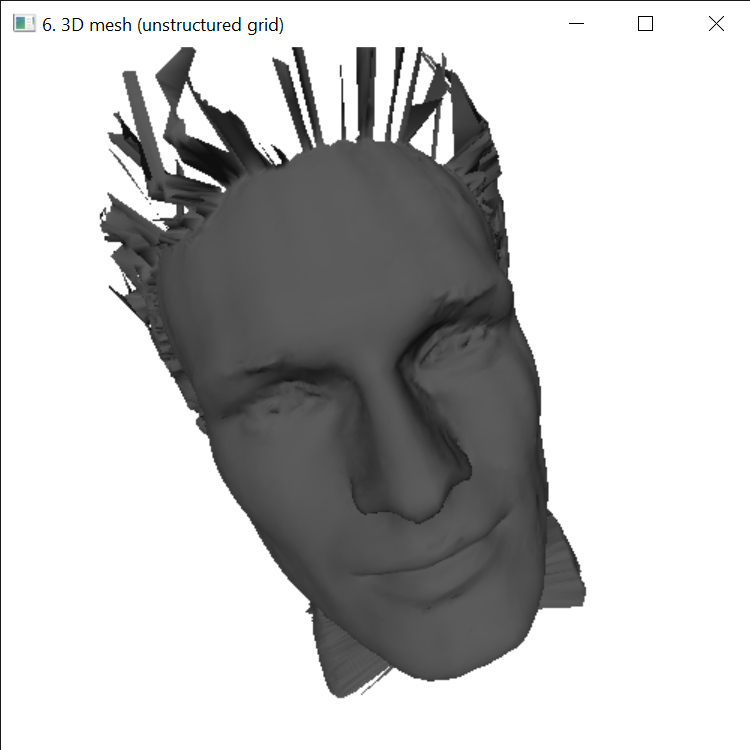
\includegraphics[width=\linewidth]{Pictures/Part3/eccHead.png}
    \caption{m303}
  \end{subfigure}
  \begin{subfigure}[b]{0.4\linewidth}
    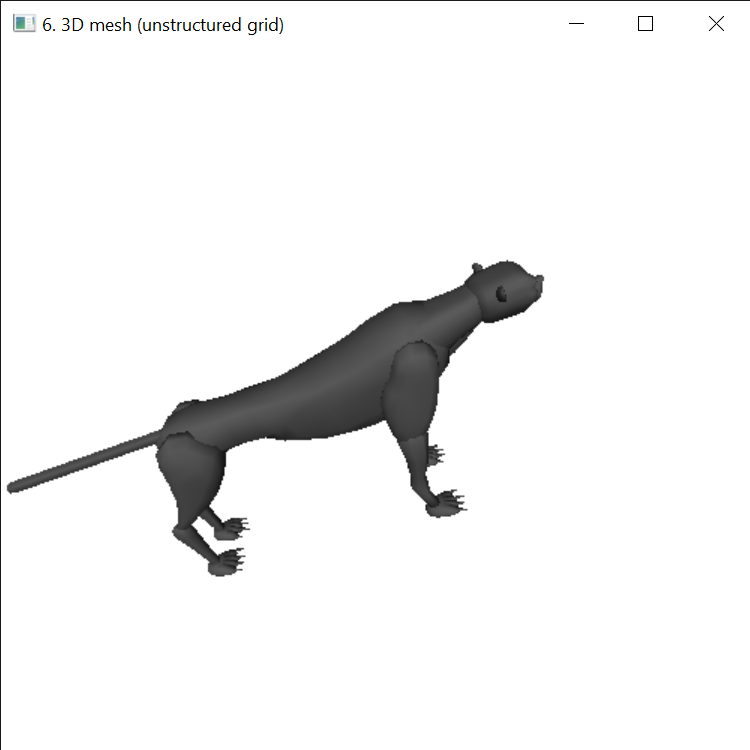
\includegraphics[width=\linewidth]{Pictures/Part3/eccLeo.png}
    \caption{m94}
  \end{subfigure}
  \caption{Two models with different eccentricity values}
  \label{fig:eccentricity}
\end{figure}
The eccentricity can go close to 0 for long objects or reach 1 for a perfect spherical form. Furthermore, this feature could also be extended to also describe the relation ratio between the other eigenvalues, $M_{e_2}$ / $M_{e_1}$ or $M_{e_3}$ / $M_{e_2}$. 

\subsubsection{Circularity and Compactness}

Circularity is the inverse of compactness, a measure which represents how compact a shape is. From this perspective, circularity shows how "circular" a shape is. In 2D, compactness is minimized by a perfect circle, where its value is 1. The formula for 2D compactness is constructed as the dimensionless ratio between a shape's perimeter ($P$) and area ($A$), with constants added to the denominator such that it produces the value 1 for a circle. The formula is the following:

\begin{equation}
C_{2D} = \frac{P^2}{4{\pi}A}
\end{equation}

Because the system requires such a metric to be used for 3D shapes, a similar formula has been derived. We begin by replacing perimeter and area with surface area ($S$) and volume ($V$), their equivalent 3D metrics:

\begin{equation}
\frac{S}{V}
\end{equation}

As the result must be dimensionless, these measures must be raised to adequate powers so that their units of measurement cancel out:

\begin{equation}
\frac{S^3}{V^2}
\end{equation}

Lastly, the constant ($x$) for the denominator must be determined by ensuring the derived formula will give 1 as the result if the shape in question is a perfect sphere:

\begin{equation}
\frac{(4\pi R^2)^3}{x(\frac{4}{3}\pi R^3)^2} = 1
\end{equation}

Solving for $x$, we obtain the result 36$\pi$. Thus, the final compactness formula is:

\begin{equation}
C_{3D} = \frac{S^3}{36\pi V^2}
\end{equation}

As mentioned at the start of this question, we use the inverse metric of compactness, circularity, due to the fact that it produces values only between 0 and 1; 1 if the shape is a sphere, and very close to 0 if the shape has a very uneven contour.

\begin{equation}
Circularity = \frac{36\pi V^2}{S^3}
\end{equation}

In the program, the two models in \textit{Figure 6} below return expected results for circularity. For the human head (a), the computation returns a value of 0.311646, much larger than the one for the leopard (b), 0.059514.

\begin{figure}[h!]
	\centering
	\begin{subfigure}[b]{0.4\linewidth}
		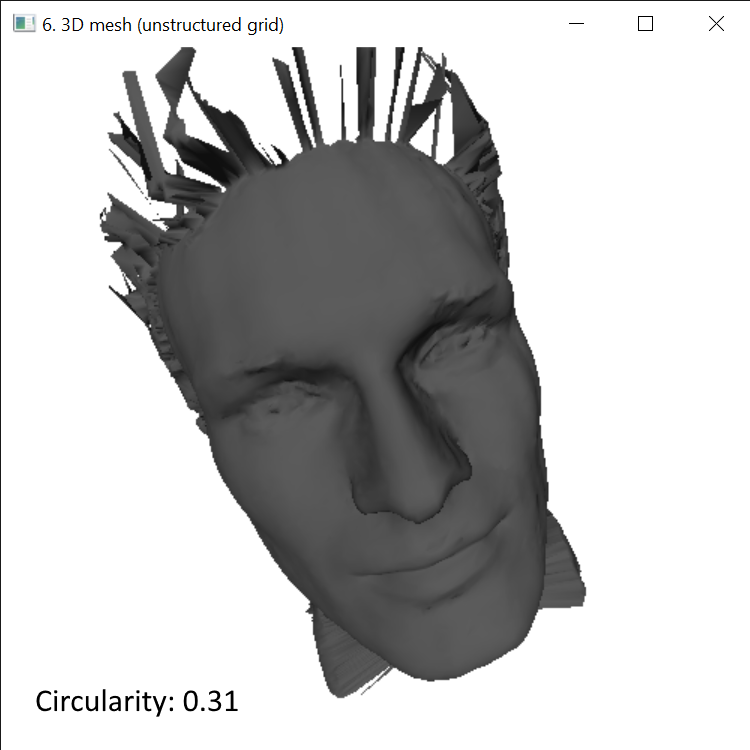
\includegraphics[width=\linewidth]{Pictures/Part3/circHead.png}
		\caption{m303}
	\end{subfigure}
	\begin{subfigure}[b]{0.4\linewidth}
		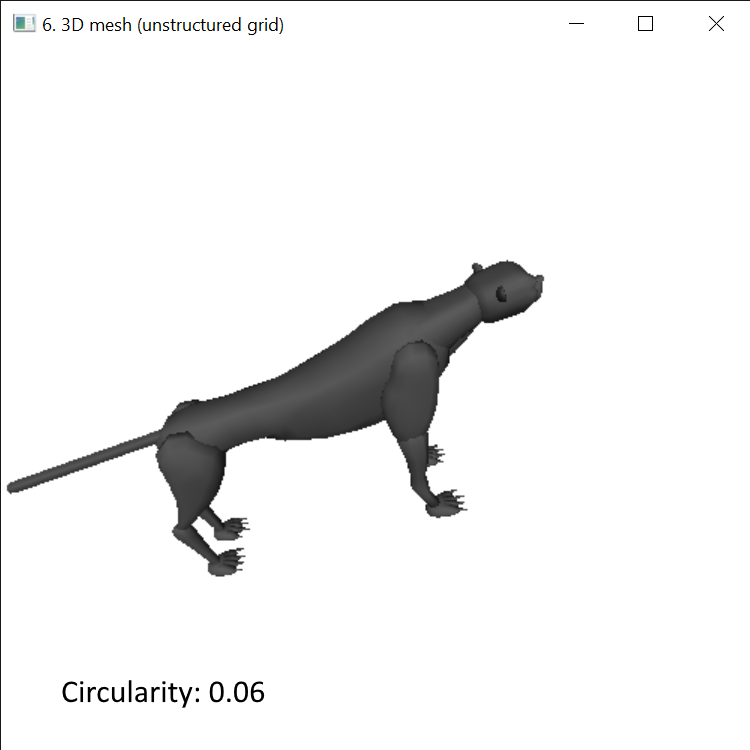
\includegraphics[width=\linewidth]{Pictures/Part3/circLeo.png}
		\caption{m94}
	\end{subfigure}
	\caption{Two models with different circularity values}
	\label{fig:circularity}
\end{figure}

\subsubsection{Diameter}
The diameter feature represents the maximum distance between two points within the shape. As our shapes have been normalized to fit within a unit cube, the maximum value for the diameter is $\sqrt{2}$, its diagonal. \\
Computing the diameter can be done through multiple approaches. The naive solution is to try every possible pair of points, resulting in a complexity of $O(n^2)$. As our shapes have around 20,000 vertices, this is not a scalable approach (a single computation can take up to 1 minute). \\
An approximation for the diameter value is obtained instead by using random samples. By sampling 2000 points from the mesh and running the brute force method, we obtain an approximation of the diameter much faster, reducing the number of steps to just $2000^2$. \\
While this approximation is fast, it's accuracy is not at all guaranteed. To increase the chances of reaching the ground truth diameter value, we can repeat this technique several times and only keep the maximum value of each approximation. Running the sampling 10 times has proven to almost always reach the ground truth within 7 seconds, down from 58 (\textit{Table 2}).

\begin{table}[h!]
	\begin{center}
		\begin{tabular}{c|l|c|c} % <-- Alignments: 1st column left, 2nd middle and 3rd right, with vertical lines in between
			\textbf{Shape} & \textbf{Method} & \textbf{Result} & \textbf{Time} \\
			\hline
\multirow{4}{3em}{m303}& Brute Force & 1.01355 & 58s\\
				  & 2000 samples & 1.01022 & $<$1s\\
				  & 5 * (2000 samples) & 1.01022 & 4s\\
				  & 10 * (2000 samples) & 1.01355 & 7s\\
			\hline
\multirow{4}{3em}{m94}& Brute Force & 1.01043 & 58s\\
				  & 2000 samples & 1.00442 & $<$1s\\
				  & 5 * (2000 samples) & 1.01043 & 4s\\
				  & 10 * (2000 samples) & 1.01043 & 7s
		\end{tabular}
	\end{center}
	\caption{t-SNE perplexity and K-L divergence results.}
	\label{Table 3,}
\end{table}

\subsubsection{Normalizing  features}
The three features bounding box volume, eccentricity, and circularity all fall in the range [0,1]. If the surface area feature is also to be normalized in this range, extent normalization has to be used by using its minimum and maximum value. However this feature has large outliers. For example the minimum of 1 and maximum of 36 is used to normalize, the distance between a surface area of 3 and 1 would become 0.0571. Even though these 2 meshes would be very different in terms of surface area, their distance does not reflect this. Therefore standardization is used for this feature, and to be consistent, it will also be used for all the other  features. 
Each new feature value will be calculated with the following formula
\begin{equation}
f'_{i,j} = \frac{f_{i,j} - \mu_i}{\delta_i},\quad i \in \{SA,BBV,ECC,DI,C\}
\end{equation}
Where $\mu_i$ is the average for feature i, $\delta_i$ the standard deviation, and $f_{i,j}$ the feature value for the $jth$ mesh. This standardization changes  the average of a feature to 0 and the standard deviation to 1. Meaning that if two different feature values differ one standard deviation from each other, there distance will be one. 

\subsection{Histogram features}
For extracting the histogram features random numbers will be generated. 
For each histogram feature they will first be generated using a minimum and maximum value based on their theoretical maximum. These results will than be used to adjust the minimum and maximum so that there wont be any bins that are universally unused. The number of bins used bins that will finally be used is set at 12.
For the histogram features several graphs are displayed showing the histograms of two different classes. This is only for an indication of how the feature might work, it certainly does not mean that the differences in values is the same for all classes, or that all classes share a similar distribution within their own class. It can however be used to show whether the feature itself works correctly. When it gives similar results for similar models, as is the case in several of the histograms. A prediction could be made that these features will help differentiate between different classes. 

\subsubsection{Sampling vertices}
Ideally for  the histogram features every possible combination of vertices should be considered. This means that for the histogram features that need two points, the number of combinations is approximately $n^2$, where $n$ is the total number of vertices. And for the triangle area, or angle, approximately $n^3$ combinations are possible. Because calculating the features for all these combinations is not possible, only a sample of these combinations will be chosen. Obviously the higher the sample size the better, it is only limited to obtain a reasonable computation time.
It is important that each combination of vertices has the same probability to be selected as a sample. This is done by randomly sampling points from the uniform distribution using the $c++$ standard library function $rand()$. If a given pair of vertices is identical the pair will be discarded. 
If for the distance between two pairs vertices n samples are generated, the probability that one of these combinations is included is $1-(\frac{1}{n^2 - 1})^{n}$. However if this same probability has to be achieved for the features that require 3 or 4 random samples, the sample size has to be increased by an order of a magnitude, i.e.
$n^2$ have to be generated. This is obviously not achievable in a reasonable time, therefore the same sample size is used for all the histogram features.
The actual sample size that is used in the system is determined by maximizing the sample size while keeping a manageable computation time. The number of samples generated are 100.000 resulting in a computation time of ~400ms. This time is considered reasonable because it allows the features of new models to be calculated in real time. When a query is submitted, the mesh has to be normalized and its features calculated, This should of course be able to be done in real time.

\subsubsection{D1 - distance to barycenter}
This feature calculates the distance between a randomly generated point and the barycenter. The distance $D$ between two vectors $u$ and $v$ is calculated as follows
\begin{equation}
D(u,v) = \sqrt{\sum\limits_{i=1}^3 (u_i - v_i)^2}
\end{equation}
The minimum distance is obviously 0, and the maximum distance is equal to the diameter of a unit cube, $\sqrt{3}$, which is an unrealistic scenario.
In order the evaluate the quality of the features, the histogram distributions of different classes will be plotted on a graph. The blue lines represent the histogram distributions of models m93, m94, m95, m96, and m97, which are all leopard like animals. And the yellow lines are models m1120, m1121, m1122, m1123, and m1124, which are air planes. These graphs will be made for each of the histogram features. 
Figure 6 indicates that the feature will not be useful for differentiating between classes. There is both large variance between the two classes, as within the classes.

\begin{figure}[h!]
    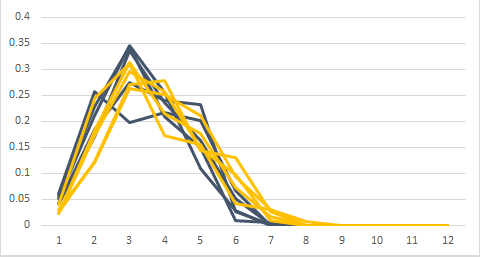
\includegraphics[width=0.7\linewidth]{Pictures/Part3/D1.png}
    \caption{Histogram distributions for feature D1 for different classes. Yellow = air planes, Blue = leopards}
  \label{fig:eccentricity}
\end{figure}

\subsubsection{D2 - distance between two points}
This time two random points are generated and the same distance function as for the D1 feature is used. The min and maximum distances are the same as the previous feature, all though the distances will generally be higher.
Figure 7 shows that the two classes have different types of distributions, however there is a lot of variation within the classes themselves.
\begin{figure}[h!]
    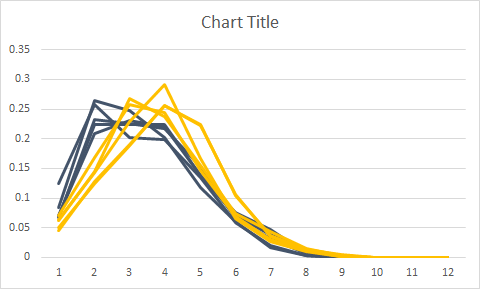
\includegraphics[width=0.7\linewidth]{Pictures/Part3/D2.png}
    \caption{Histogram distributions for feature D2 for different classes. Yellow = air planes, Blue = leopards}
  \label{fig:eccentricity}
\end{figure}

\subsubsection{D3 - area of a random triangle}
To get a random triangle three random points are generated. The area of this triangle is calculated the same way as was done for calculating the total surface area. The square root of this value is than added to the histogram, because the other two features were the lengths of line segments.
Figure 8 shows a difference between the two classes, however there is also some variation within the classes. 

\begin{figure}[h!]
    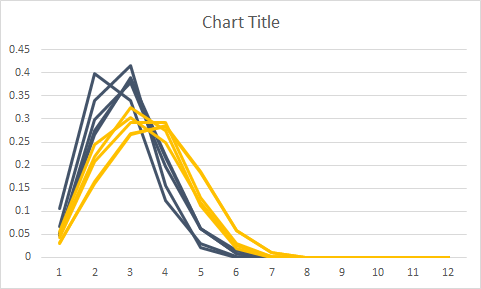
\includegraphics[width=0.7\linewidth]{Pictures/Part3/D3.png}
    \caption{Histogram distributions for feature D3 for different classes. Yellow = air planes, Blue = leopards}
  \label{fig:eccentricity}
\end{figure}

\subsubsection{D4 - are of a random tetrahedron}
Four random points $a$, $b$, $c$, and $d$ are generated that together will make the tetrahedron. The formula used for calculating the volume is:
\begin{equation}
V(a,b,c,d) = \frac{|(a - d) \cdot ((b - d) \times (c - d))|}{6}
\end{equation}
Than the cube root of this value is taken, because it is a volume and the other features are the lengths of line segments. Figure 9 a significant difference between distributions of air planes and leopards. Furthermore the in class differences are minimally. Therefore this might indicate that D4 is a good feature. 
\begin{figure}[h!]
    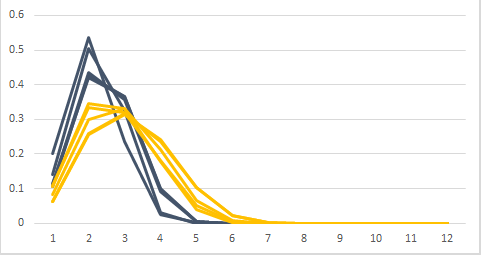
\includegraphics[width=0.7\linewidth]{Pictures/Part3/D4.png}
    \caption{Histogram distributions for feature D3 for different classes. Yellow = air planes, Blue = leopards}
  \label{fig:eccentricity}
\end{figure}

\subsubsection{A3 - angle between 3 random vertices}
The last histogram features uses three random points $u$, $v$, and $w$ to calculate the angle between them. These three points create a triangle that has three angles, however the order in which they are generated determines which angle is chosen. Therefore all three possible angles are calculates, and the maximum of those is chosen. For each angle the distance is chosen by using two vectors that share a similar point. For example, the vectors $a = v-u$ and $b = w-u$ give one possible angle of the triangle. The formula used for calculating an angle given two vectors is as follows:
\begin{equation}
Angle(a,b) = atan2(N(a \times b), (a \cdot b))
\end{equation}
Where N gives the euclidean norm of a vector, and atan2 the angle in the euclidean plane. The minimum value that the angle could be is 0, and the maximum is $\pi$.
In figure 10 it can be seen that the two classes are quite dissimilar, however one of the air planes seems to be an outlier compared to the rest of its class.

\begin{figure}[h!]
    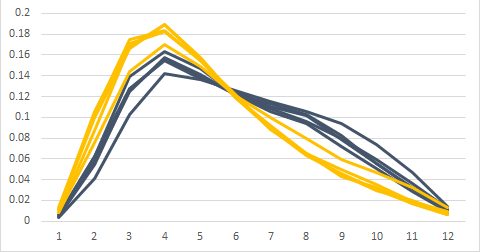
\includegraphics[width=0.7\linewidth]{Pictures/Part3/A3.png}
    \caption{Histogram distributions for feature A3 for different classes. Yellow = air planes, Blue = leopards}
  \label{fig:eccentricity}
\end{figure}

\subsection{Feature vector}
A model $i$ can be represented in the system using its feature vector $F_i$. This is created by combining all of the previously discussed features $f_{i,j}$.
\begin{equation}
F_i = \{f_{1,j}, f_{2,j}, .. , f_{10,j}\}
\end{equation}
Each $f_{i,j}$ is a list of $k$ values, where $k$ is 1 for the scalar values and 12 for the histogram values.

\begin{table}
\begin{center}
\begin{tabular}
{ l | l | l | l | l | l}
i & feature name & k & min & max\\ \hline
1 & surface area & 1 & -0.919356 & 19.06002 \\
2 & bounding box volume & 1 & -1.178278 & 3.28805\\
3 & eccentricity & 1 & -0.810042 & 4.419431\\
4 & circularity & 1 & -0.549875 & 6.57143\\
5 & diameter & 1 & -3.472866 & 5.231975\\
6 & distance to barycenter & 12 & 0 & 1.060660\\
7 & distance between two points & 12 & 0 & $\sqrt{2}$\\
8 & area of a random triangle & 12 & 0 & 0.848528 \\
9 & area of a random tetrahedron & 12 & 0 & 0.565685\\
10 & angle between 3 random vertices & 12 & 0.942478 & $\pi$\\
\end{tabular}
\end{center}
\caption{Feature vector format and standardized extreme values.}
\label{Table 2, }
\end{table}
The feature vector is thus a list of 65 values.


\section{Matching}
All the features discussed in the previous section are calculated for each mesh and put in a single feature vector $x = (x_1,...,x_n)$ where each $x_i$ is a single feature. To compare different meshes the distance is to be calculated between their two feature vector. If feature vector $x$ is compared with a different feature vector $y = (y_1,...y_3$, each of their features will be compared individually and the sum of these distances will be regarded as the distance between the two feature vectors.

\subsection{Distance calculation}
Each feature has $m$ values, for  features $m = 1$ because it only has value, for histograms $m$ is equal to the number of bins of that histogram. The distance function $L_(x,y)$ gives the total euclidean distance between two feature vectors $x$ and $y$
\begin{equation}
L(x,y) = \left(\sum\limits_{i=1}^nd(x_i,y_i)^2\right)^{1/2}
\end{equation}
Where $d$ is a function that calculates the distance between two features
\begin{equation}
d(x_i,y_i) = \frac{\left(\sum\limits_{j=1}^m|x_{i,j}-y_{i,j}|^2\right)^{1/2}}{m}
\end{equation}
Where $x_{i,j}$ is the jth value of the ith feature of feature vector $x$, the same case for $y$. The sum of all the distances between feature values is divided by $m$ so that each feature has the same weight, i.e. a histogram with 8 values should not be weighted 8 time as much as a scalar feature which has only 1 value.  

\subsection{Query result}
These distances are calculated for each mesh in the database, obviously excluding the the query item, if it exists. The result is thus a list of distances for a query item i $L_i = {d_1, ... d_k}$, where $k$ is the number of items in the database, and is ordered in ascending order. With an input query size $s$ the first $s$ elements of $L$ are than returned as the query result. An alternative approach by using the KNN algorithm is discussed in the following section. 

\subsection{kd-tree}
The system when used by the end user should return a number of relevant models $k$ as specified by the user. In the previous described method the distances are being sorted first resulting in a time complexity of $\mathcal{O}(n\log{}n)$, alternatively for a small size of k, instead of sorting the result it could simply be traversed k times and finding a new nearest neighbour each time, this has a time complexity of $\mathcal{O}(kn)$. In this system the size of the dataset is not so high that this becomes unreasonable, however to be able to scale up with a larger dataset a search structure can be created. The data structure used is called a kd-tree and is a way to partition the data to allow for fast searches. The cost of creating such a tree is $\mathcal{O}(n\log{}n)$, however this can be precomputed and stored server side so that this overhead cost is irrelevant for a user. Searching for the k nearest neighbours in this tree has an average time complexity of $\mathcal{O}(k\log{}n)$, which thus greatly accelerates the search process. \\
The library used in this system for creating and searching kd-trees is ANN. In addition to the previously mentioned search, ANN has the functionality of an approximate search, which accelerates the search in exchange for a user specified loss in accuracy. In this system however, because the number of models and dimensions is small, the exact k nearest neighbours are returned instead. 

\section{Dimensionality reduction}
In order to assess the quality of our feature vectors, a means to visualize the entire dataset and how distinguishable each class is from the others is desirable. As it is impossible to directly plot our 65-dimensional feature vectors into a scatter plot, the dimensionality reduction technique known as t-Distributed Stochastic Neighbor Embedding (t-SNE) has been used to transcribe our feature space into two dimensions. (van der Maaten \& Hinton, 2008) describe the technique in detail. This section discusses how this was achieved, then the resulting plot is shown. 

\subsection{Perplexity Parameter}
T-SNE takes as input, aside from the data itself, three parameters: the number of desired dimensions (2 in our case), the dimensionality of the data (65 dimensions) and perplexity. The latter is defined in (van der Maaten \& Hinton, 2008) as 2 to the power of the Shannon entropy of the probability distribution represented by our multidimensional space. In practice, however, perplexity is a parameter that must be experimented with to determine the best results. \newline
Several values between 0 and 100 have been tested in an attempt to select the one that minimizes the "error" reported by the algorithm, which is actually the Kullback-Leibler divergence between the original multidimensional data and the 2D result. The table below displays the results:

\begin{table}[h!]
	\begin{center}
		\begin{tabular}{l|c} % <-- Alignments: 1st column left, 2nd middle and 3rd right, with vertical lines in between
			\textbf{Perplexity} & \textbf{K-L Divergence}\\
			\hline
			25.0 & 0.927\\
			50.0 & 0.915\\
			75.0 & 0.905\\
			100.0& 0.909
		\end{tabular}
	\end{center}
\caption{t-SNE perplexity and K-L divergence results.}
\label{Table 3,}
\end{table}

\subsection{Resulting Plot}

However, t-SNE is not deterministic, as it initializes its gradient function randomly. Instead of finding a perfect perplexity, it could be more appropriate to run the algorithm multiple times with the same perplexity and choosing the result with minimal error. After several attempts, the lowest error obtained was 0.660 on 100.0 perplexity. This can be seen in Figure 11. \\
\begin{figure}[!h]
	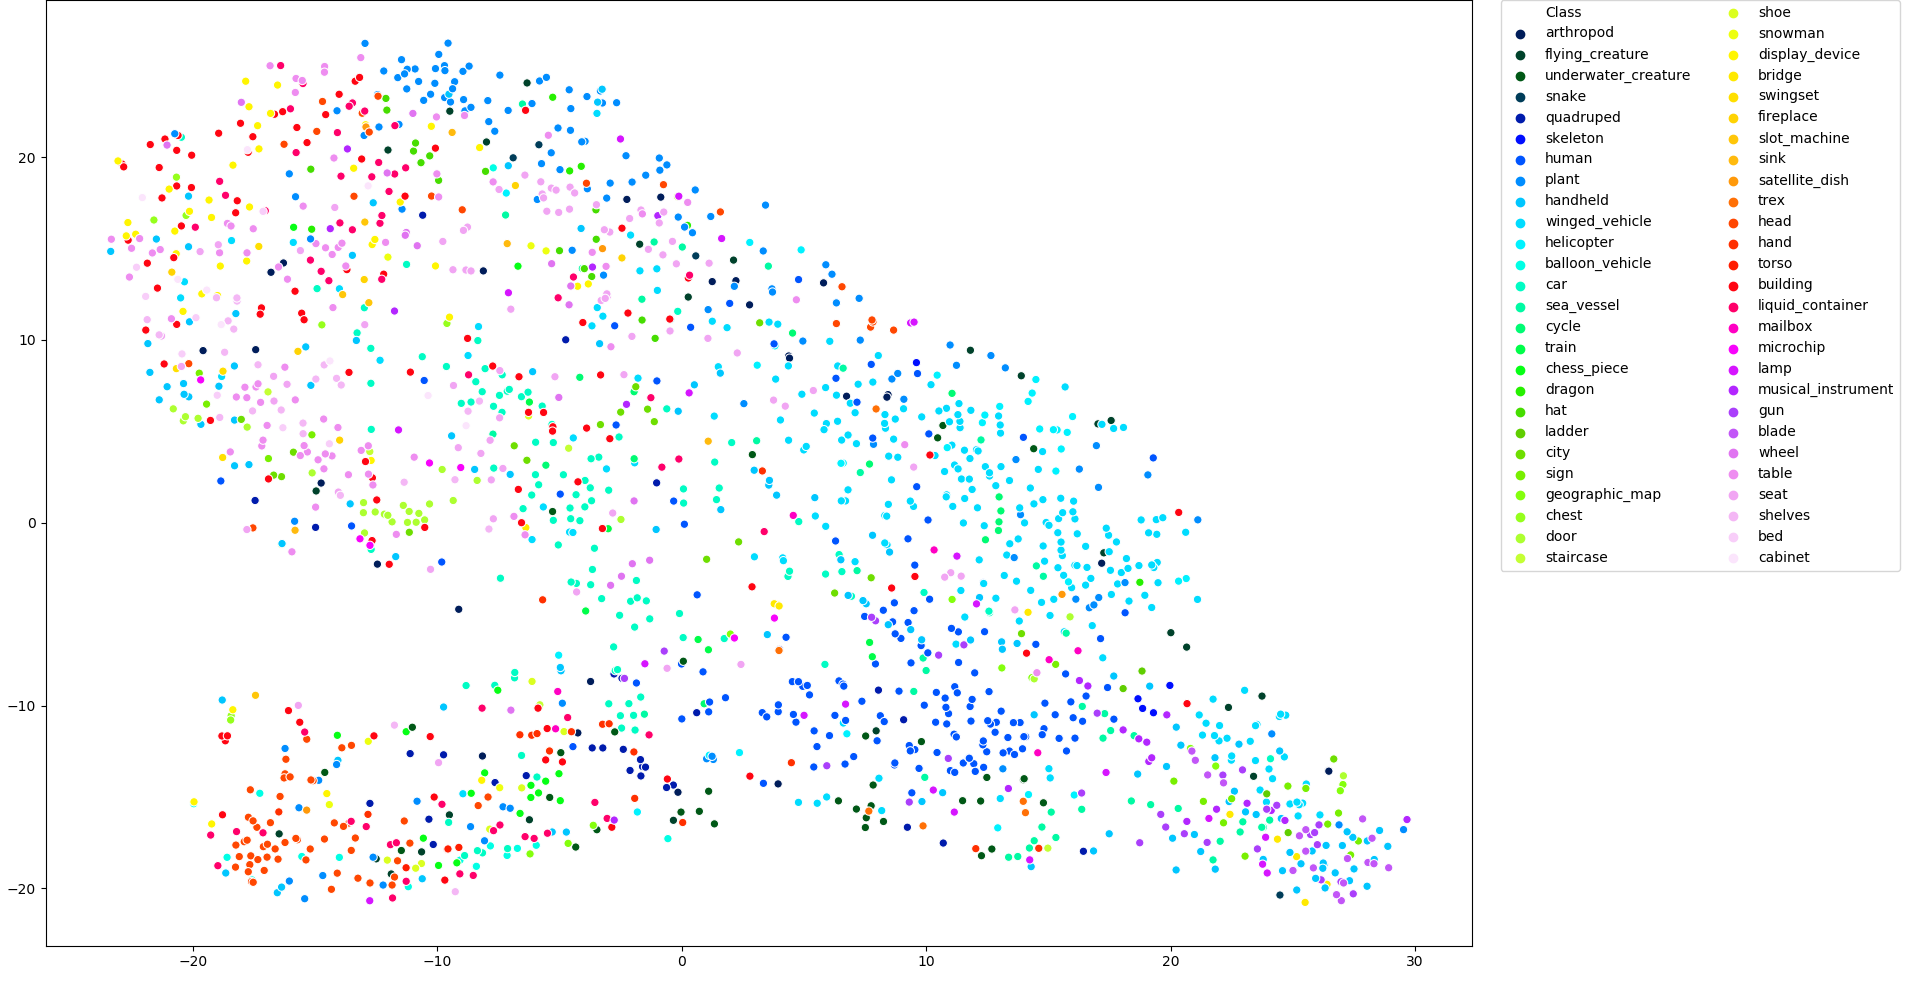
\includegraphics[width=1\linewidth]{Pictures/perp100err0-660.png}
	\label{fig:fig1}
	\caption{t-SNE plot on feature vector space: 100.0 perplexity and 0.660 error}
\end{figure}

While the figure is hard to read due to the large amount of points and classes, some information that confirms the feature values are not random can be derived from it. For example, the clusters of humans and winged vehicles are fairly well delimited, and so are the clusters for heads and doors.

\section{Evaluation}
The final step is to evaluate the performance of the retrieval system. This is done by analysing the query result $Q$ which as a list of items ${x_1,...,x_s}$, where s is the size of the query and each x is an item in the database. As was explained in the matching section, this list is ordered on ascending distance to the query item $l$. First of, there are several values that describe a query result, namely the true positives (TP), false positives (FP), true negatives (TN), and false negatives (FP). TP is the number of items with the correct class label in a query, FP the number of wrong items in a query, TN the number of wrong items not in the query result, and FN the number of correct items not in query.
\\ 
$TP = |\{y \in Q\, |\, c_y = c_l\}|$\\
$FP = s - TP$\\
$TN = k - TP - FP - FN$\\
$FN = N_{c_l} - TP$\\
\\
Where $c_i$ is the class label of item $i$, $k$ the number of items in the dataset, and $N_{c_l}$ the number of items in the class of query item l.  

\subsection{Evaluation metric}
There are many evaluation metrics that can be used. Furthermore, there are different aspects of the system for which the performance can be evaluated. For example the performance for a single item in the dataset, the average performance of a class, and the overall performance of the program. In the evaluation of this system the performance for each item will be calculated and from those measurements the class averages, and overall performance will be derived. The overall performance is calculated as the average of all items, not an average of all classes.\\
The performance metric chosen are mean average precision (MAP) and precision at k. Regarding the query result for a model, the model for which the query result is generated is not included in its own query result. The distance of a model to itself will always be 0 and would thus give a misleading precision it were to be included. The definition of these performance metric and why they are chosen is discussed in the following two sections.

\subsubsection{MAP}
Two interesting evaluation metrics are precision and recall. Precision shows how many of the returned items in the query are of the correct class, while recall shows how many of the correct class are represented in the query. The problem with recall however is that it is highly dependent on the size of the query. A query of size 1 can never have a recall of 1, assuming that the class size is higher than 1. Therefore the recall is not a useful performance metric for this system, because it gives little insight. A large query size will result in a high recall and a low query size in low recall. The more interesting metric is precision whose definition is given below.
\begin{equation}
P = \frac{TP}{TP+FP}
\end{equation}
Another problem that arrives is what query size the evaluation metric should be calculated for. A universal query size is undesirable, because there are large discrepancies between the sizes of different classes. A class with only five items will have a terrible performance when the query size is set to 100, because the maximum precision is $\frac{5}{100}$. 
Furthermore, even for a specific class, choosing the query size is an arbitrary decision. Therefore the Mean Average Precision (MAP) is used.
The query result that is returned by the matching algorithm is an ordered list of ascending distance values of size $d$, where $d$ is the size of the database. The MAP for a class is the mean of all the average precisions of its models query results. The average precision for the query result of a given model is defined as:
\begin{equation}
AvgP = \frac{\sum_{k=1}^{n}(P(k) \cdot rel(k)}{m}
\end{equation}
Where rel(k) is the indicator function and is 1 if the kth item in the query result has the correct label and 0 otherwise, and m is the number of models in the relevant class. The MAP for a class is than the mean of all these average precision values.\\
MAP  might punish some classes too much when it contains an outlier. If it does than for each model in the class the outlier will yield a precision close to 0. In this case it might be possible that even a perfect system cannot obtain a precision of 1, because of an outlier or even a wrongly sampled mesh. Furthermore calculating precision for items that are very far in the query result can be useless when the user only wants a small result. For example a user would not want to look at more than 20 models, therefore only the first 20 results would be relevant. If a system would return 20 items that have the correct class label, but the other 20 items in the class appear in the back of the query result, the average precision would be close to 0.5, while the returned query is a perfect result for the user. Despite these downsides of the MAP it is still chosen as a strict metric to judge the performance of the entire system. One of the upsides of MAP is that it considers the position of the correct classes, which is not the case for the regular precision. 

\subsubsection{Precision at k}
In addition to the MAP another performance metric is introduced, the precision at k. For this a value for k has to be decided, which will be the length of the query result. Than for this smaller sized query its precision will be calculated. As was previous discussed, a user might only want to look at a certain number of items, precision at k than measures how many correct items the user will see. In the evaluations in this report the value for k will be set at 10. However because some classes contain less than 10 models, k well be $min(k,n_c-1)$ where $n_c - 1$ is the number of models in class c, excluding the model that is queried for. 
A downside of precision at k is that it does not account for the position of models. For example a result query with only the first five items being the correct class and a second result query with only  the last five items being the correct class, will have the same precision at k. Intuitively however the first query result is better. 

\begin{minipage}{\linewidth}
\begin{center}
\begin{tabular}
{ l | l | l | l}
\textbf{class name} & \textbf{MAP} & \textbf{Precision at k} & \textbf{Observed model count} \\ \hline
winged vehicle & 0.416308 & 0.666527 & 239 \\ \hline
balloon vehicle & 0.116555 & 0.14375 & 16 \\ \hline
helicopter & 0.123383 & 0.22 & 35 \\ \hline
arthropod & 0.0545013 & 0.103704 & 27 \\ \hline
human & 0.394029 & 0.648993 & 149 \\ \hline
trex & 0.0641384 & 0.0666667 & 6 \\ \hline
flying creature & 0.0340165 & 0.05 & 26 \\ \hline
quadruped & 0.120444 & 0.232258 & 31 \\ \hline
snake & 0.0491144 & 0.0833333 & 4 \\ \hline
underwater creature & 0.131797 & 0.231429 & 35 \\ \hline
blade & 0.20551 & 0.257895 & 19 \\ \hline
head & 0.292354 & 0.496104 & 77 \\ \hline
hand & 0.11159 & 0.176471 & 17 \\ \hline
skeleton & 0.409468 & 0.4 & 5 \\ \hline
torso & 0.549304 & 0.5 & 4 \\ \hline
bridge & 0.103303 & 0.1 & 10 \\ \hline
building & 0.08743 & 0.161225 & 98 \\ \hline
chess piece & 0.203151 & 0.276471 & 17 \\ \hline
chest & 0.0761211 & 0.047619 & 7 \\ \hline
city & 0.0492937 & 0.0894737 & 19 \\ \hline
display device & 0.111166 & 0.18 & 40 \\ \hline
door & 0.301497 & 0.439286 & 28 \\ \hline
dragon & 0.0524088 & 0.0666667 & 6 \\ \hline
fireplace & 0.0110214 & 0 & 6 \\ \hline
bed & 0.0463207 & 0.0535714 & 8 \\ \hline
cabinet & 0.0725405 & 0.0833333 & 9 \\ \hline
seat & 0.159862 & 0.327273 & 77 \\ \hline
shelves & 0.172277 & 0.276923 & 26 \\ \hline
table & 0.167187 & 0.342308 & 78 \\ \hline
geographic map & 0.0562935 & 0.1 & 11 \\ \hline
gun & 0.112295 & 0.178571 & 28 \\ \hline
hat & 0.152967 & 0.2125 & 16 \\ \hline
ladder & 0.0446827 & 0 & 4 \\ \hline
lamp & 0.0475397 & 0.0863636 & 22 \\ \hline
liquid container & 0.0873931 & 0.19661 & 59 \\ \hline
mailbox & 0.022605 & 0 & 7 \\ \hline
microchip & 0.0683838 & 0.047619 & 7 \\ \hline
musical instrument & 0.0932159 & 0.15 & 22 \\ \hline
plant & 0.194478 & 0.391111 & 135 \\ \hline
satellite dish & 0.0023526 & 0 & 4 \\ \hline
sea vessel & 0.098209 & 0.229545 & 44 \\ \hline
shoe & 0.0831799 & 0.107143 & 8 \\ \hline
sign & 0.0635423 & 0.1125 & 16 \\ \hline
sink & 0.00389432 & 0 & 4 \\ \hline
slot machine & 0.0768283 & 0 & 4 \\ \hline
snowman & 0.15229 & 0.166667 & 6 \\ \hline
swingset & 0.0991632 & 0 & 4 \\ \hline
staircase & 0.00529275 & 0 & 7 \\ \hline
handheld & 0.0996813 & 0.202459 & 122 \\ \hline
car & 0.24536 & 0.483636 & 110 \\ \hline
cycle & 0.125922 & 0.138462 & 13 \\ \hline
train & 0.0980175 & 0.0952381 & 7 \\ \hline
wheel & 0.0992868 & 0.158824 & 17 \\ \hline
\textbf{total} & \textbf{0.200032} & \textbf{0.343097} & \textbf{1796} \\ \hline
\end{tabular}
\end{center}
\begin{center}
Table ?. Performance evaluation using MAP and precision at k (k=10)
\end{center}
\end{minipage}

\subsection{Dissimilar classes}
The performance results show that there is a large discrepancy between performances of different classes. The worst classes even have a precision at k of 0, meaning that for none of the models in its class the result query gave even a single relevant model in the first 10 results. This leads to the questions of what causes this bad result, and what can be done to improve performance for this class. For the first question four of the models of the staircase class are shown in figure 11. It is clear that the overall shapes of these model is very different, this leads to their feature values being very different as well. \\
Some characteristics of a staircase are present in these pictures, namely the large number of 90 degree edges leading to the top. A feature could be added that would encapsulate this characteristic so that all these models will have a distance of 0 for this feature. However even in this case, all the other feature values will be very different, making it very unlikely that their overall distances will be small enough to yield good results.

\begin{figure}[h!]
  \centering
  \begin{subfigure}[b]{0.2\linewidth}
    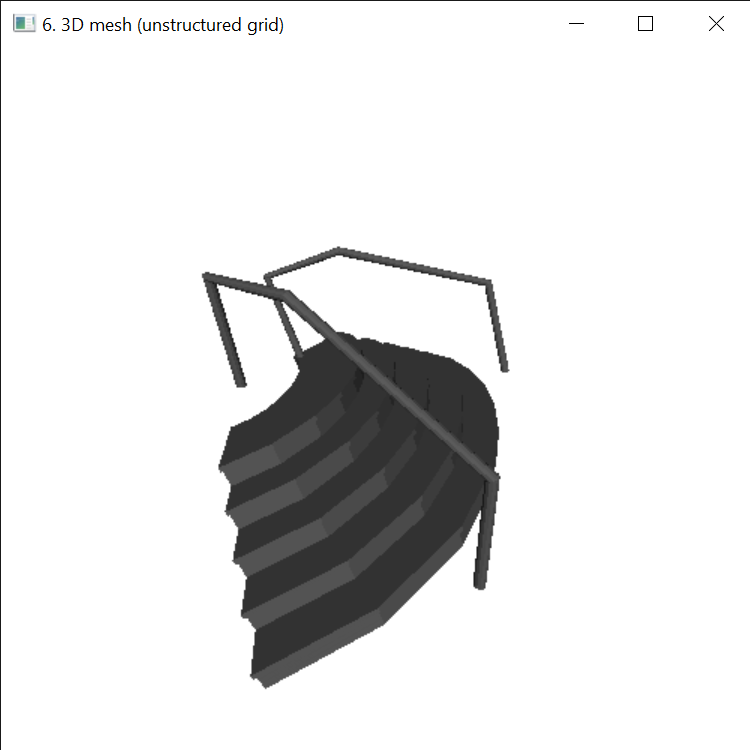
\includegraphics[width=\linewidth]{Pictures/Evaluation/staircaseClass/stair1.png}
  \end{subfigure}
  \begin{subfigure}[b]{0.2\linewidth}
    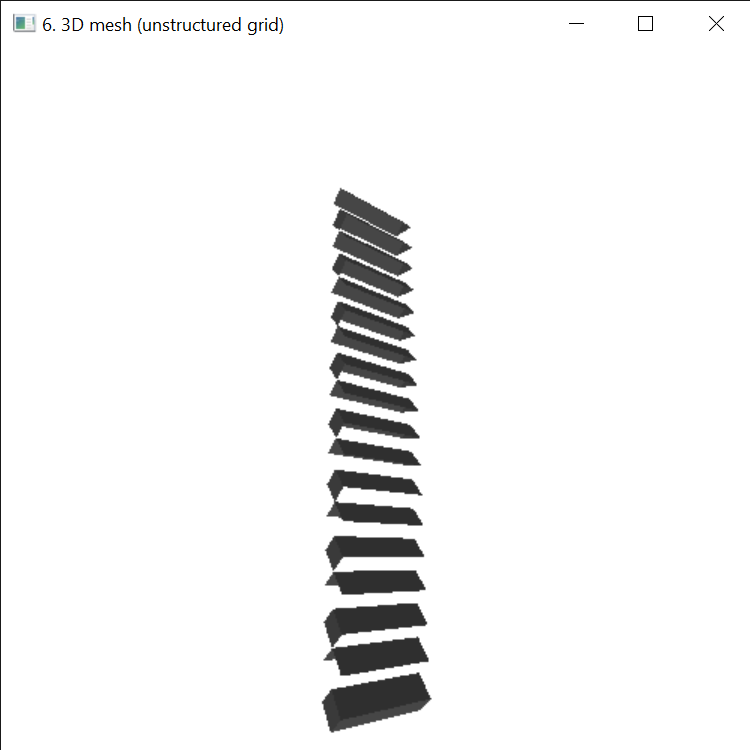
\includegraphics[width=\linewidth]{Pictures/Evaluation/staircaseClass/stair2.png}
  \end{subfigure}
  \begin{subfigure}[b]{0.2\linewidth}
    \includegraphics[width=\linewidth]{Pictures/Evaluation/staircaseClass/stair3.png}
  \end{subfigure}
  \begin{subfigure}[b]{0.2\linewidth}
    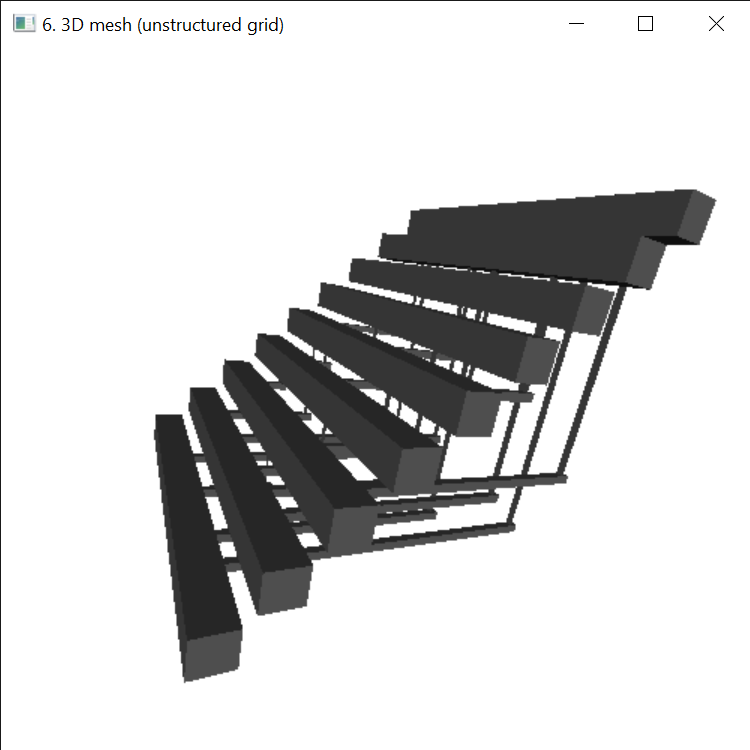
\includegraphics[width=\linewidth]{Pictures/Evaluation/staircaseClass/stair4.png}
  \end{subfigure}
  \caption{Models m1733, m1734, m1735, and m1736 of the staircase class.}
  \label{fig:bunny}
\end{figure}

Looking at another bad performing class, the mailboxes, a less obvious difference in models is visible. The models look a lot more alike, however their distances are still too large. The seemingly small differences in shapes have a large impact on their feature values. For example the first and fourth mailboxes are shorter than the second and fourth. Furthermore the volume of the actual box is different in each model. Finally there are some more small differences, such as the rectangular shape below the box in the fourth model, and the extended rectangles in the third shape. \\
It could thus be said that even though these models look alike, their actual shapes are still too different for the system. The small differences lead in feature value differences that are too large. Both the mailbox class and the staircase class have a precision at k of 0, however the mailbox class has an MAP value four times that of the staircase class, meaning that the relative distances of mailboxes are smaller than the staircases. This makes sense because intuitively one would say that the mailboxes are more similar to each other than the staircases. 

\begin{figure}[h!]
  \centering
  \begin{subfigure}[b]{0.2\linewidth}
    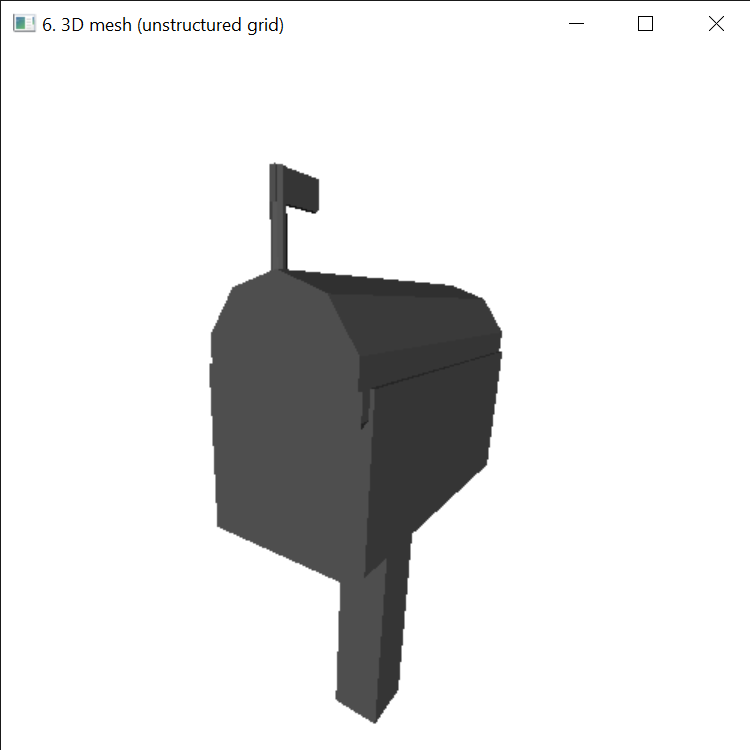
\includegraphics[width=\linewidth]{Pictures/Evaluation/mailboxClass/stair1.png}
  \end{subfigure}
  \begin{subfigure}[b]{0.2\linewidth}
    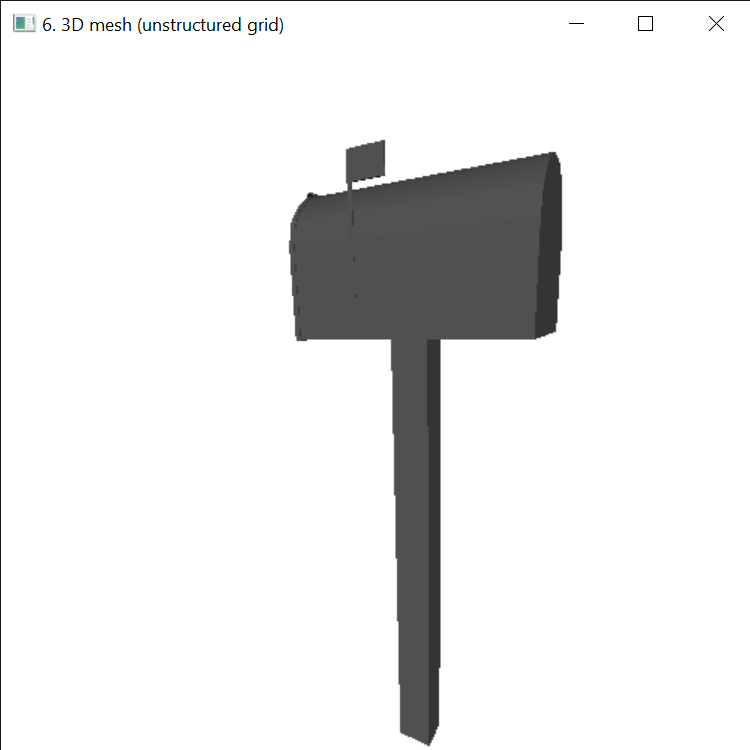
\includegraphics[width=\linewidth]{Pictures/Evaluation/mailBoxClass/stair2.png}
  \end{subfigure}
  \begin{subfigure}[b]{0.2\linewidth}
    \includegraphics[width=\linewidth]{Pictures/Evaluation/mailBoxClass/stair3.png}
  \end{subfigure}
  \begin{subfigure}[b]{0.2\linewidth}
    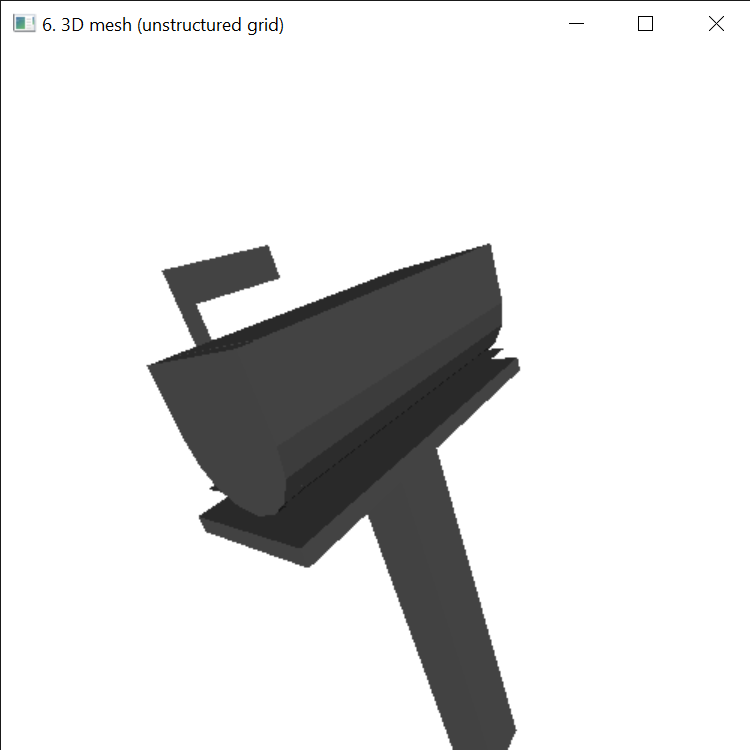
\includegraphics[width=\linewidth]{Pictures/Evaluation/mailBoxClass/stair4.png}
  \end{subfigure}
  \caption{Models m515, m516, m517, and m517 of the mailbox class.}
  \label{fig:bunny}
\end{figure}

\subsection{Query examples}
In this section several query results are shown for several different classes. Firstly, we will query for a model from the quadruped class which has a MAP of 0.12, and precision at k of 0.23. For this specific model five out of nine models are of the same class. Three of these wrong models, the hands, can be explained by them having a similar elongated shape and their fingers resembling legs. The turtle does not have a similar shape however it does also have four legs.  \\
Secondly a query result for a model of the flying creature class is shown, which has an MAP of 0.034, and precision at k of 0.05. In this case only two out of the nine models of the query result are of the same class. Six of these however are air planes and have a very similar shape. The ship is the only of these models that is an unreasonable result. The system thus returns models that are arguably very similar to the input shape, all though not from the same class \\
Finally the query result for one of the best performing classes, humans, shows a perfect query result. The good results for humans show that they are somewhat clustered in the dataset. This means for a certain amount of models they exist in the middle of the clusters and thus all of its neighbors are other humans. \\

\begin{figure}[h!]
  \centering
  \begin{subfigure}[b]{0.09\linewidth}
    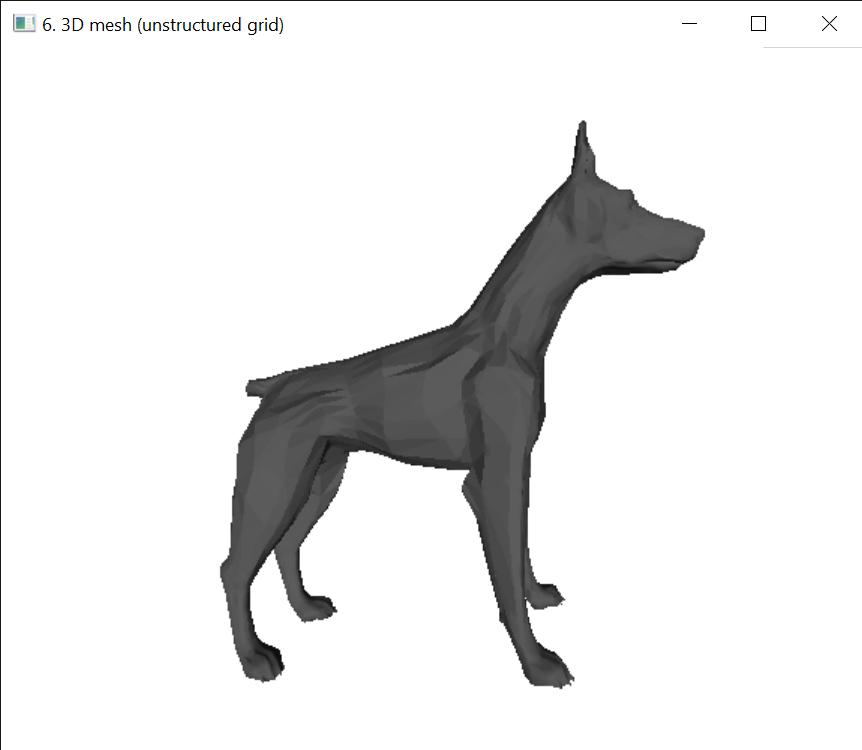
\includegraphics[width=\linewidth]{Pictures/Evaluation/m92/m92.png}
    \caption*{d=0}
  \end{subfigure}
  \begin{subfigure}[b]{0.09\linewidth}
    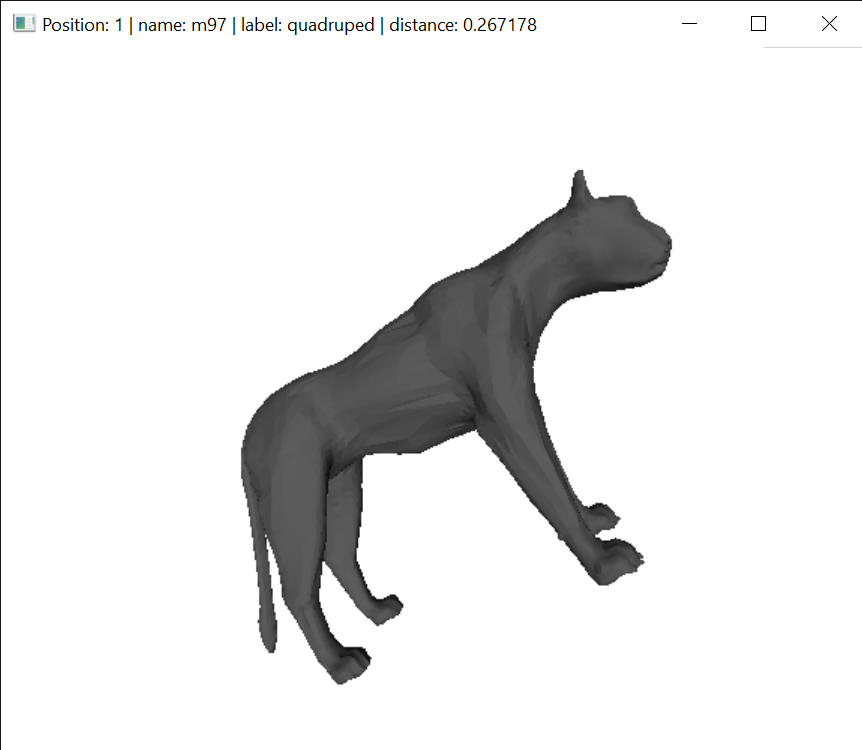
\includegraphics[width=\linewidth]{Pictures/Evaluation/m92/pos1.png}
    \caption*{d=0.27}
  \end{subfigure}
  \begin{subfigure}[b]{0.09\linewidth}
    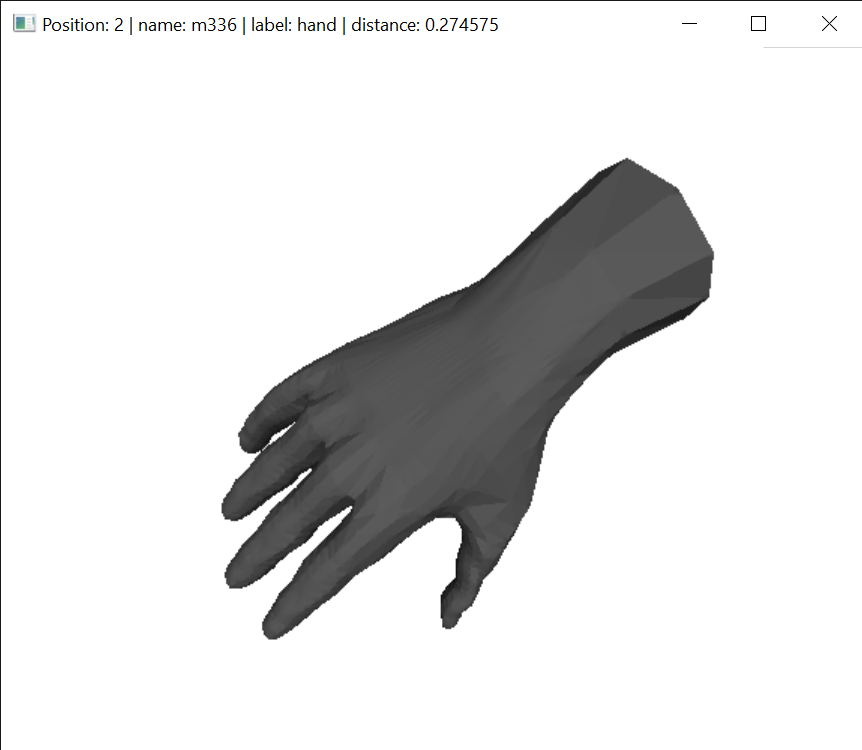
\includegraphics[width=\linewidth]{Pictures/Evaluation/m92/pos2.png}
    \caption*{d=0.27}
  \end{subfigure}
  \begin{subfigure}[b]{0.09\linewidth}
    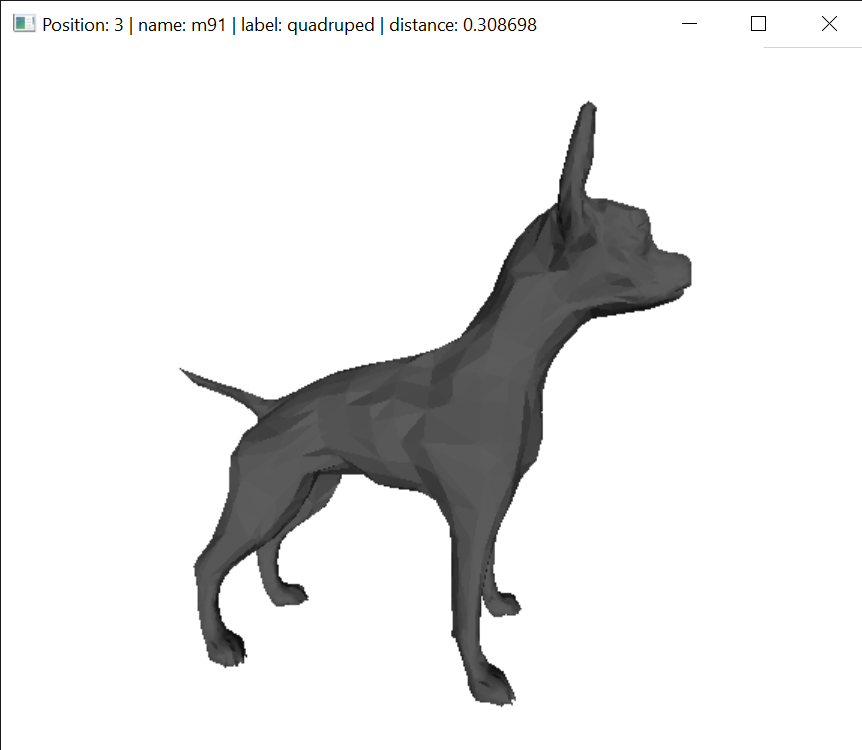
\includegraphics[width=\linewidth]{Pictures/Evaluation/m92/pos3.png}
    \caption*{d=0.31}
  \end{subfigure}
  \begin{subfigure}[b]{0.09\linewidth}
    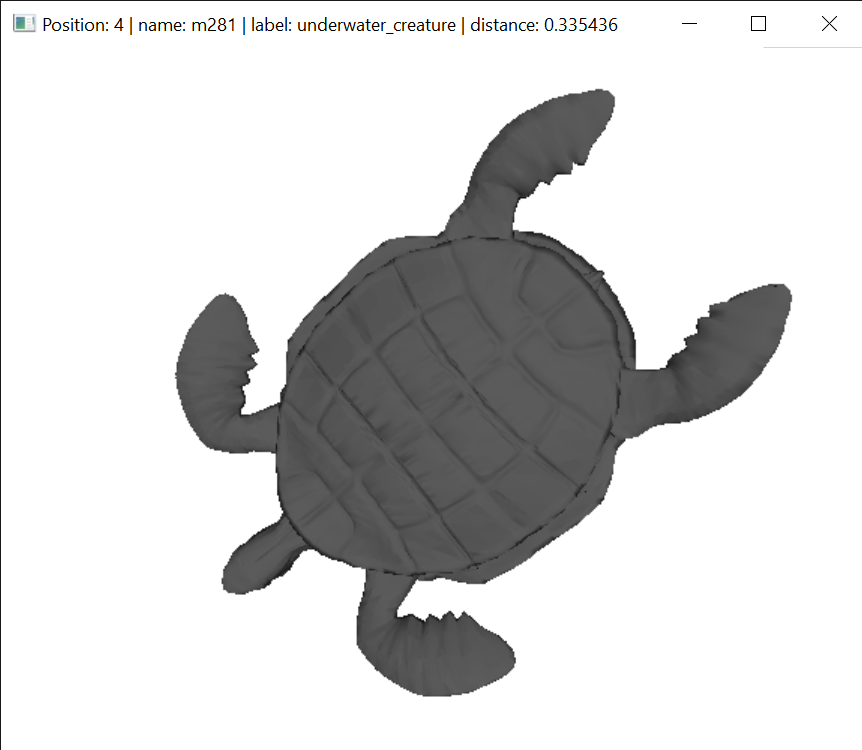
\includegraphics[width=\linewidth]{Pictures/Evaluation/m92/pos4.png}
    \caption*{d=0.34}
  \end{subfigure}
  \begin{subfigure}[b]{0.09\linewidth}
    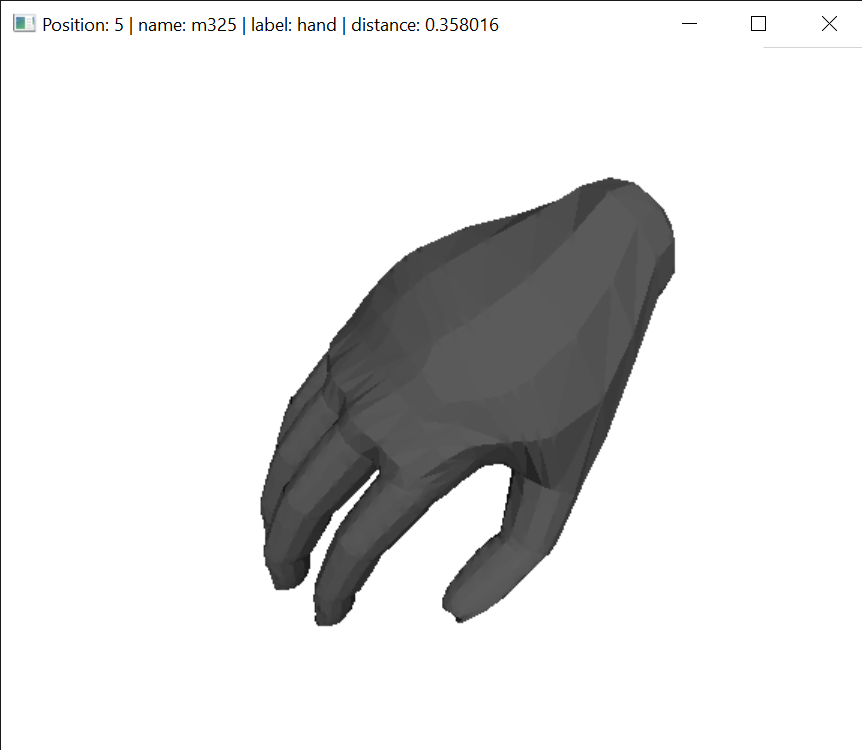
\includegraphics[width=\linewidth]{Pictures/Evaluation/m92/pos5.png}
    \caption*{d=0.36}
  \end{subfigure}
  \begin{subfigure}[b]{0.09\linewidth}
    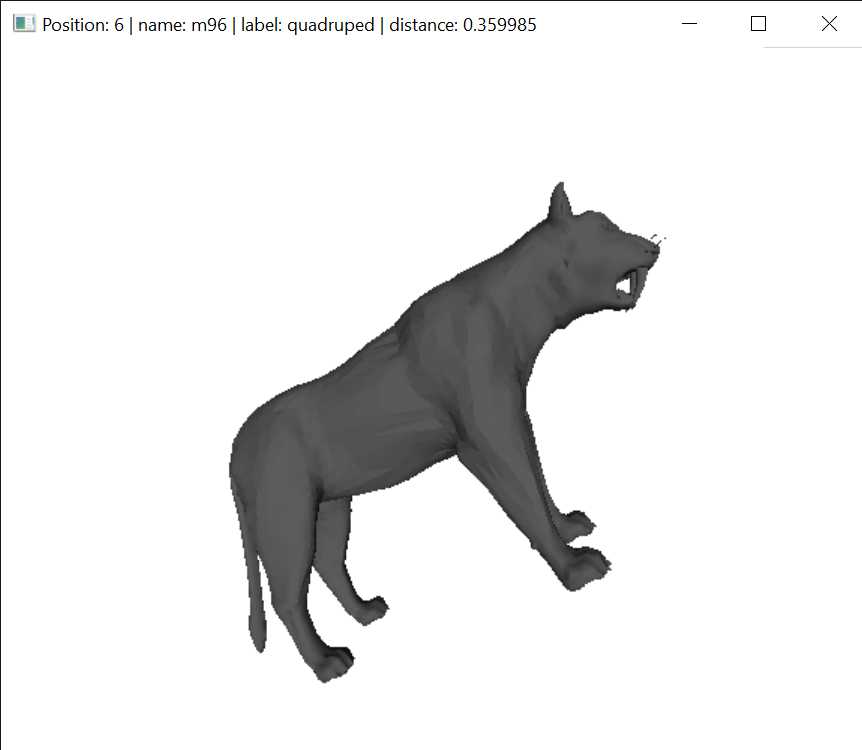
\includegraphics[width=\linewidth]{Pictures/Evaluation/m92/pos6.png}
    \caption*{d=0.36}
  \end{subfigure}
  \begin{subfigure}[b]{0.09\linewidth}
    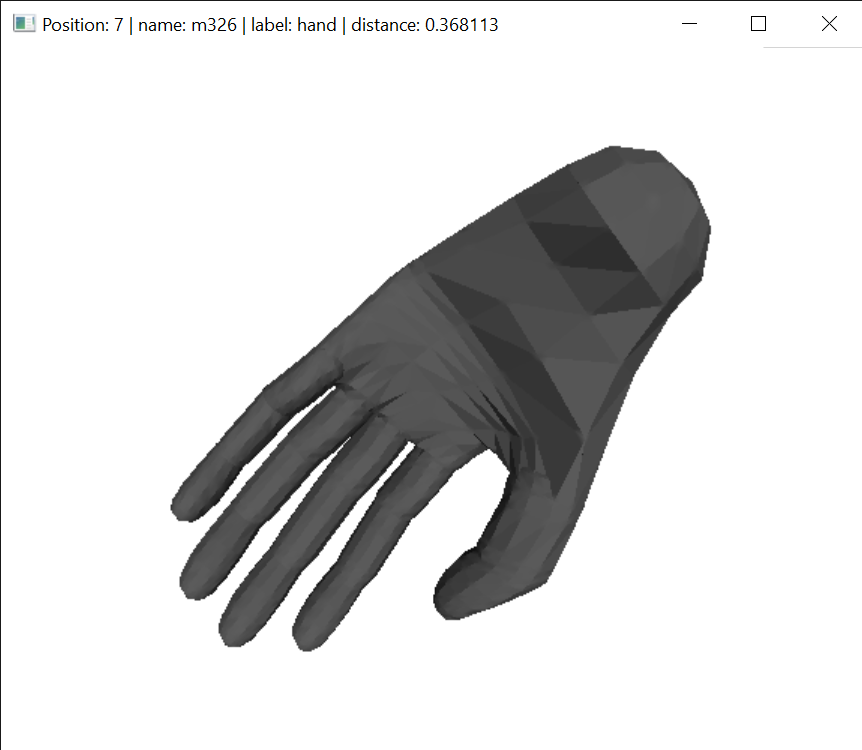
\includegraphics[width=\linewidth]{Pictures/Evaluation/m92/pos7.png}
    \caption*{d=0.37}
  \end{subfigure}
  \begin{subfigure}[b]{0.09\linewidth}
    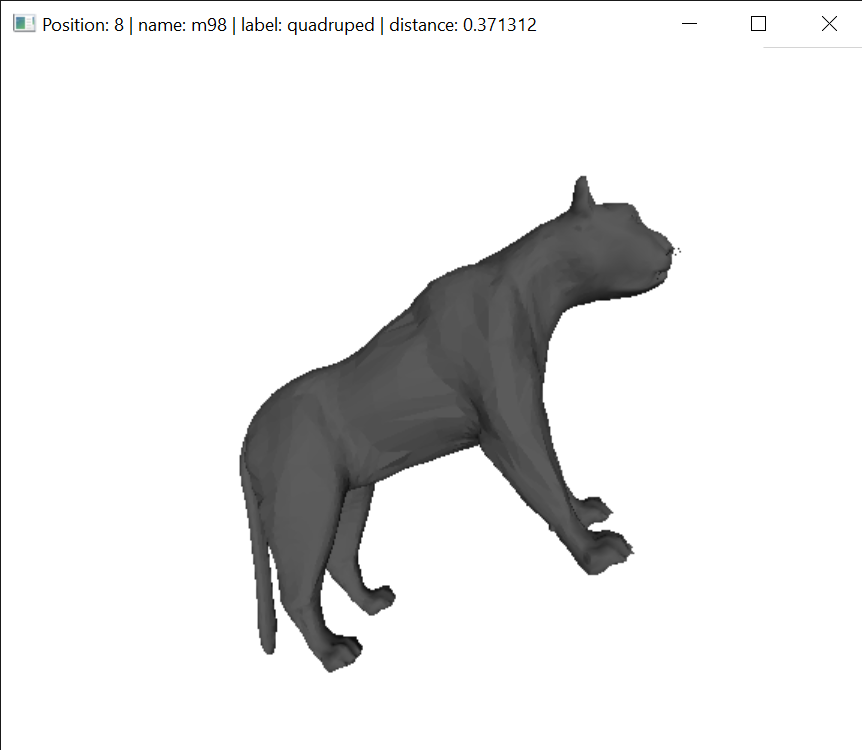
\includegraphics[width=\linewidth]{Pictures/Evaluation/m92/pos8.png}
    \caption*{d=0.37}
  \end{subfigure}
  \begin{subfigure}[b]{0.09\linewidth}
    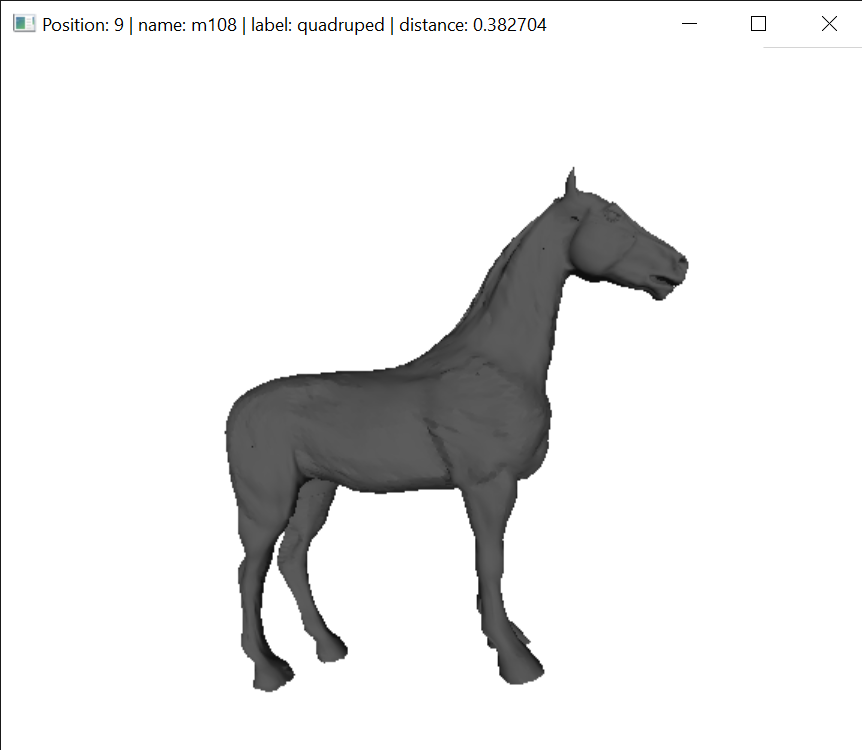
\includegraphics[width=\linewidth]{Pictures/Evaluation/m92/pos9.png}
    \caption*{d=0.38}
  \end{subfigure}

  \centering
  \begin{subfigure}[b]{0.09\linewidth}
    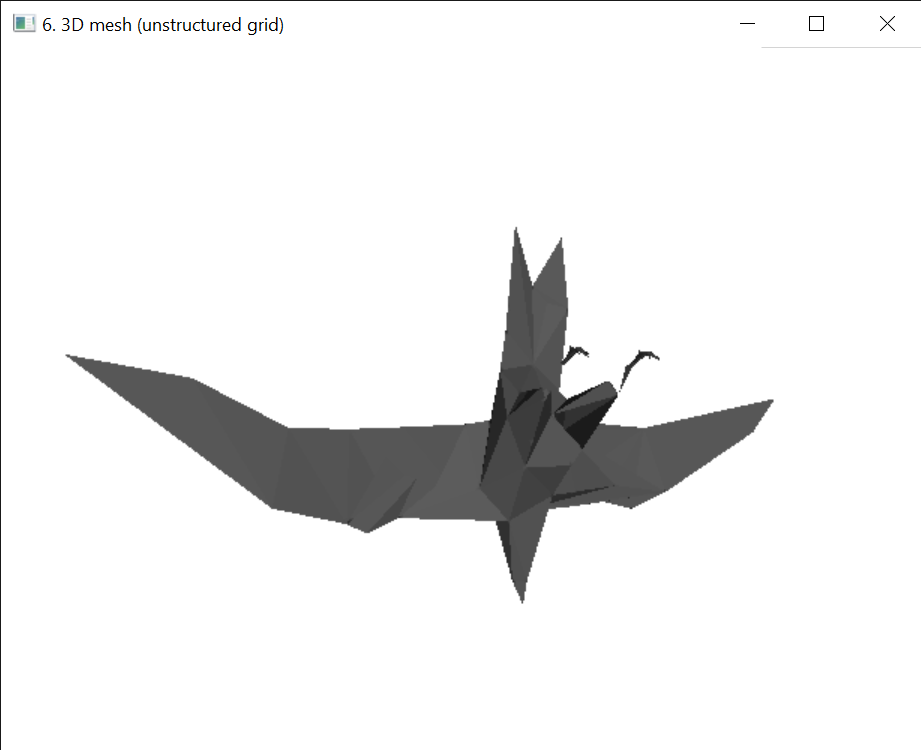
\includegraphics[width=\linewidth]{Pictures/Evaluation/m42/m42.png}
    \caption*{d=0}
  \end{subfigure}
  \begin{subfigure}[b]{0.09\linewidth}
    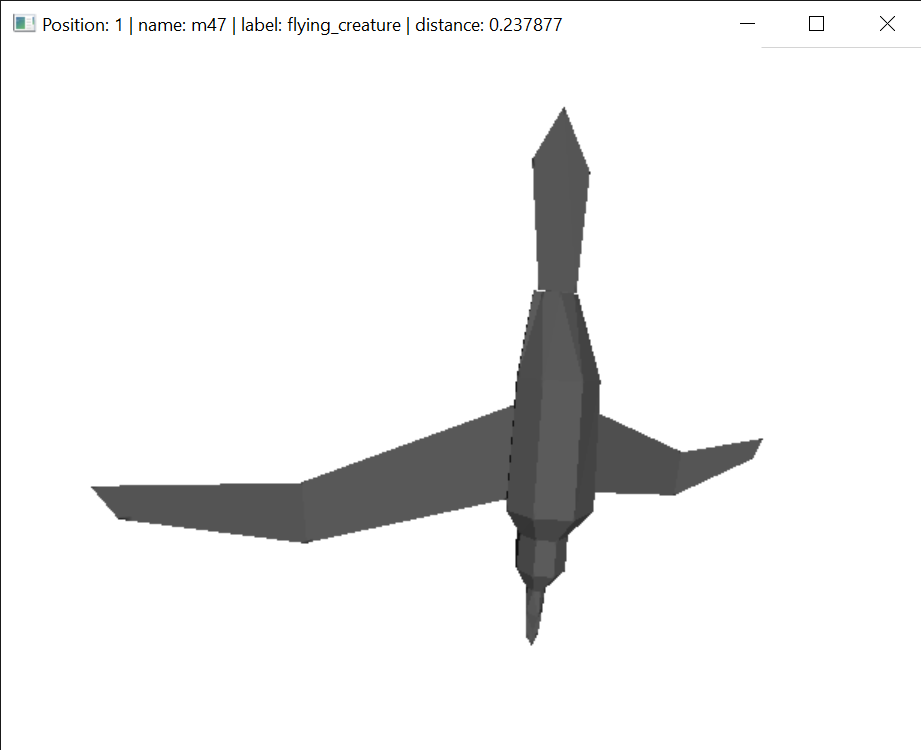
\includegraphics[width=\linewidth]{Pictures/Evaluation/m42/pos1.png}
    \caption*{d=0.24}
  \end{subfigure}
  \begin{subfigure}[b]{0.09\linewidth}
    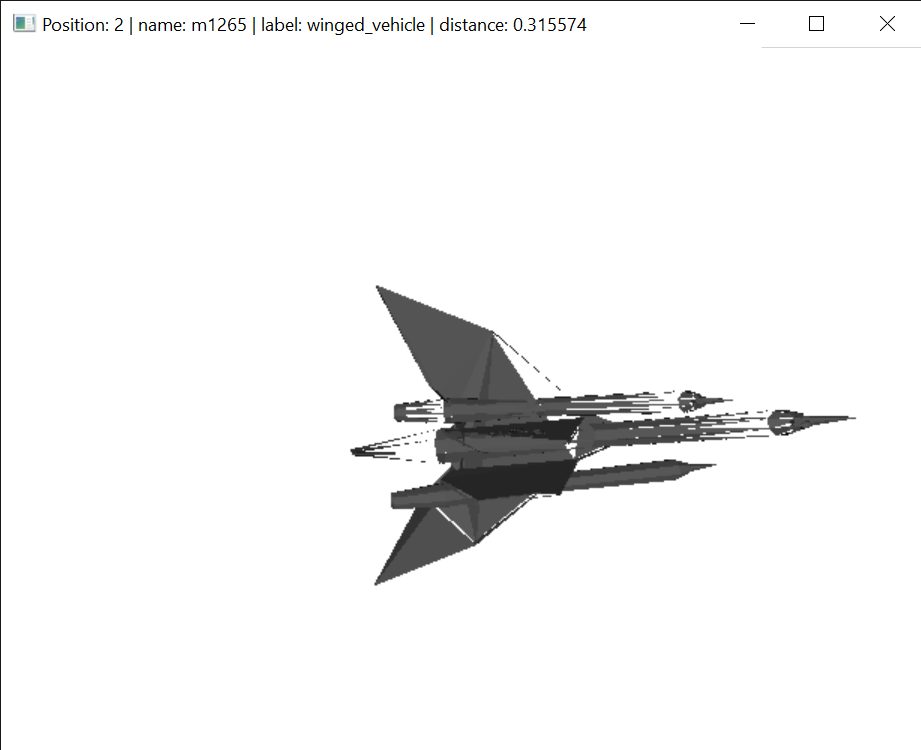
\includegraphics[width=\linewidth]{Pictures/Evaluation/m42/pos2.png}
    \caption*{d=0.32}
  \end{subfigure}
  \begin{subfigure}[b]{0.09\linewidth}
    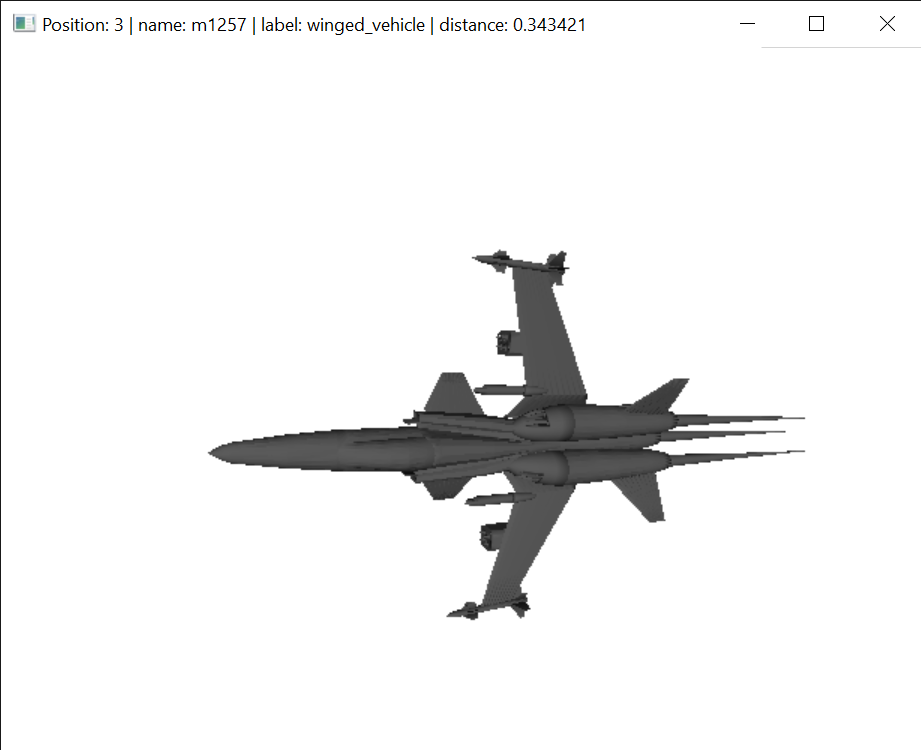
\includegraphics[width=\linewidth]{Pictures/Evaluation/m42/pos3.png}
    \caption*{d=0.34}
  \end{subfigure}
  \begin{subfigure}[b]{0.09\linewidth}
    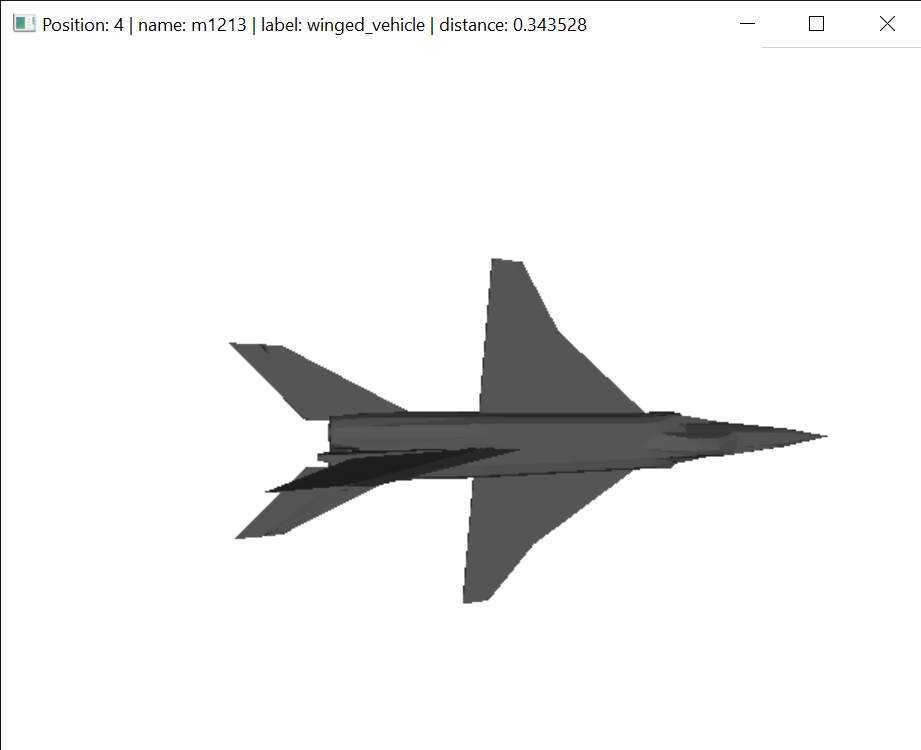
\includegraphics[width=\linewidth]{Pictures/Evaluation/m42/pos4.png}
    \caption*{d=0.34}
  \end{subfigure}
  \begin{subfigure}[b]{0.09\linewidth}
    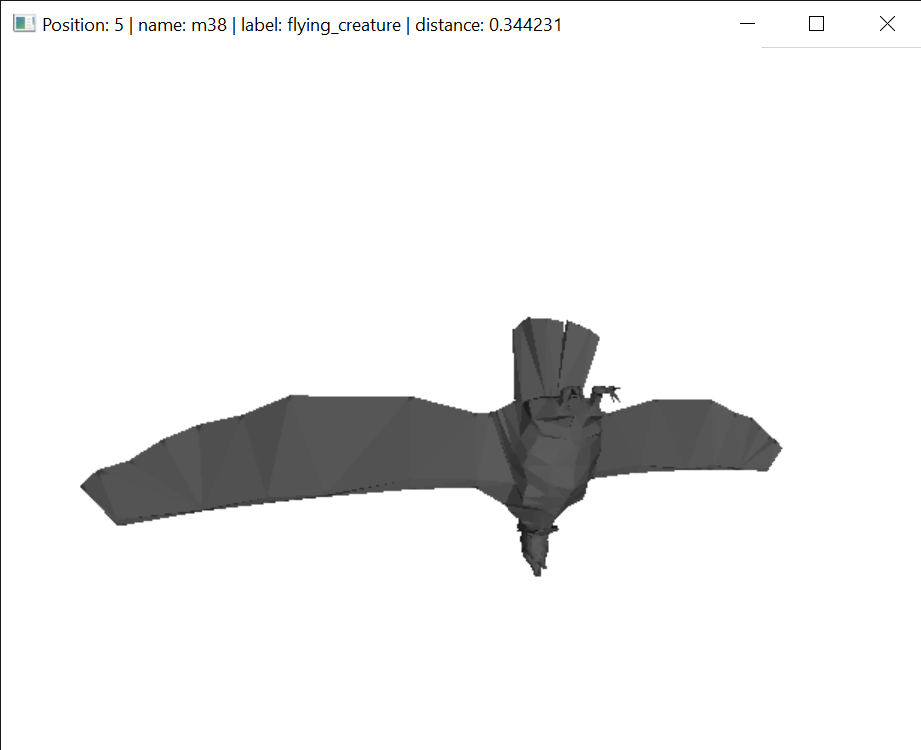
\includegraphics[width=\linewidth]{Pictures/Evaluation/m42/pos5.png}
    \caption*{d=0.34}
  \end{subfigure}
  \begin{subfigure}[b]{0.09\linewidth}
    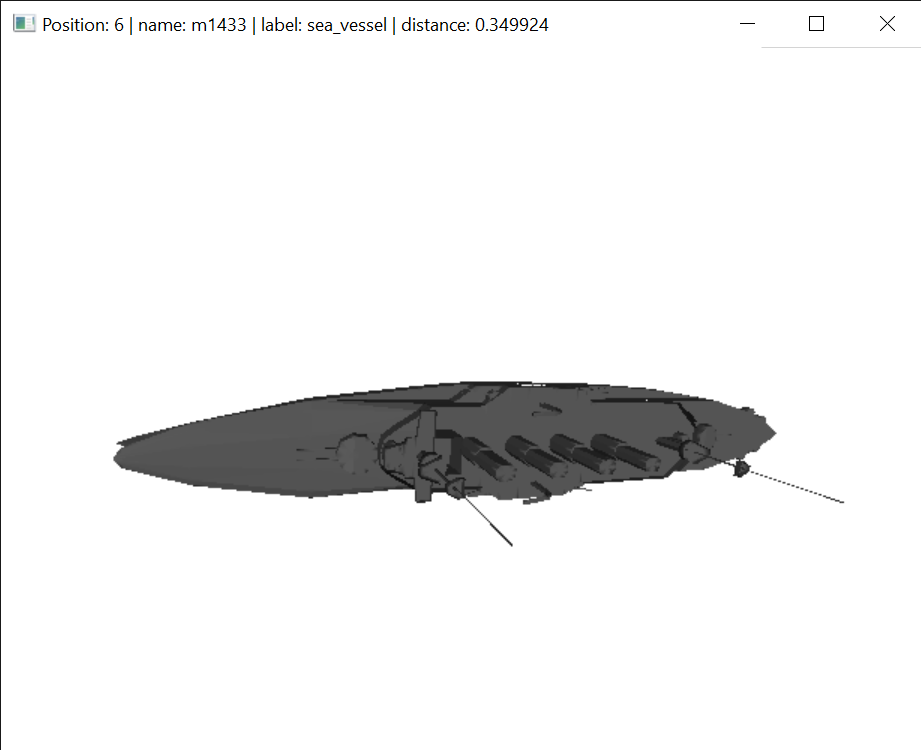
\includegraphics[width=\linewidth]{Pictures/Evaluation/m42/pos6.png}
    \caption*{d=0.35}
  \end{subfigure}
  \begin{subfigure}[b]{0.09\linewidth}
    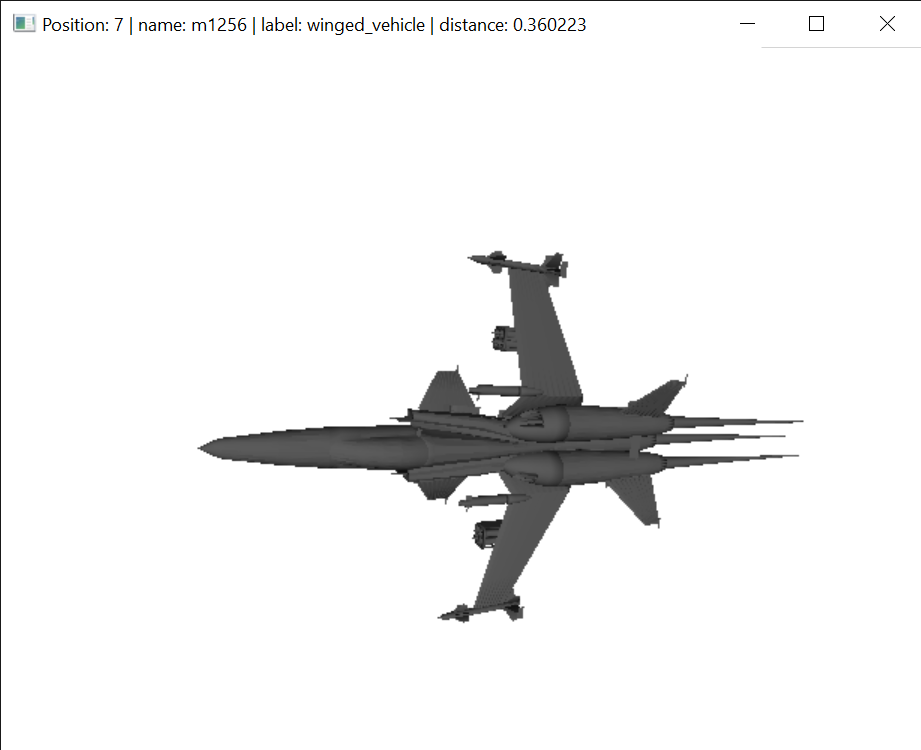
\includegraphics[width=\linewidth]{Pictures/Evaluation/m42/pos7.png}
    \caption*{d=0.36}
  \end{subfigure}
  \begin{subfigure}[b]{0.09\linewidth}
    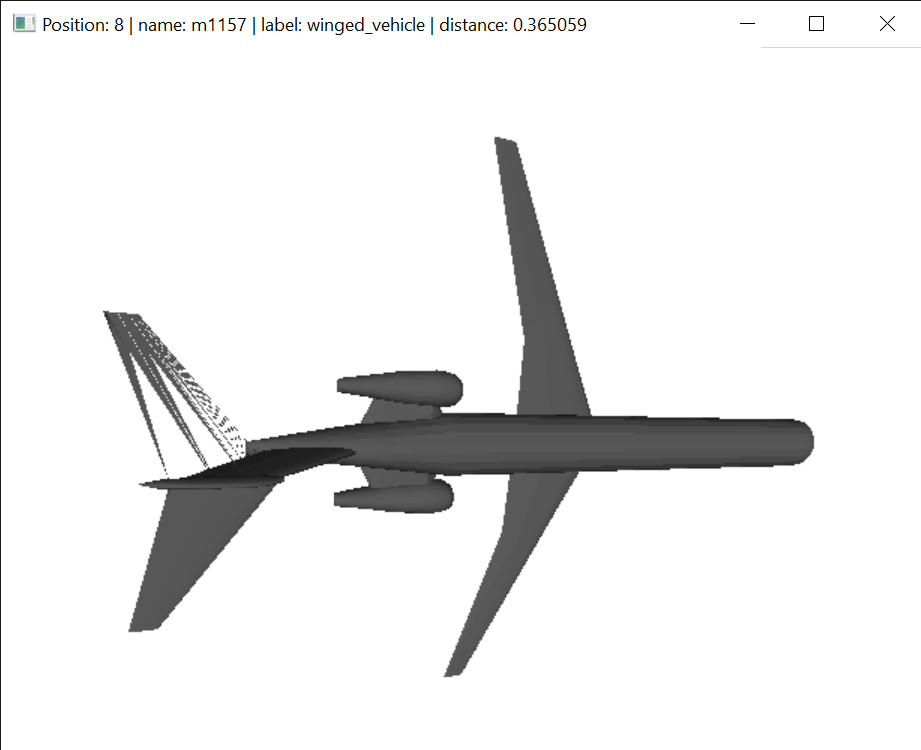
\includegraphics[width=\linewidth]{Pictures/Evaluation/m42/pos8.png}
    \caption*{d=0.37}
  \end{subfigure}
  \begin{subfigure}[b]{0.09\linewidth}
    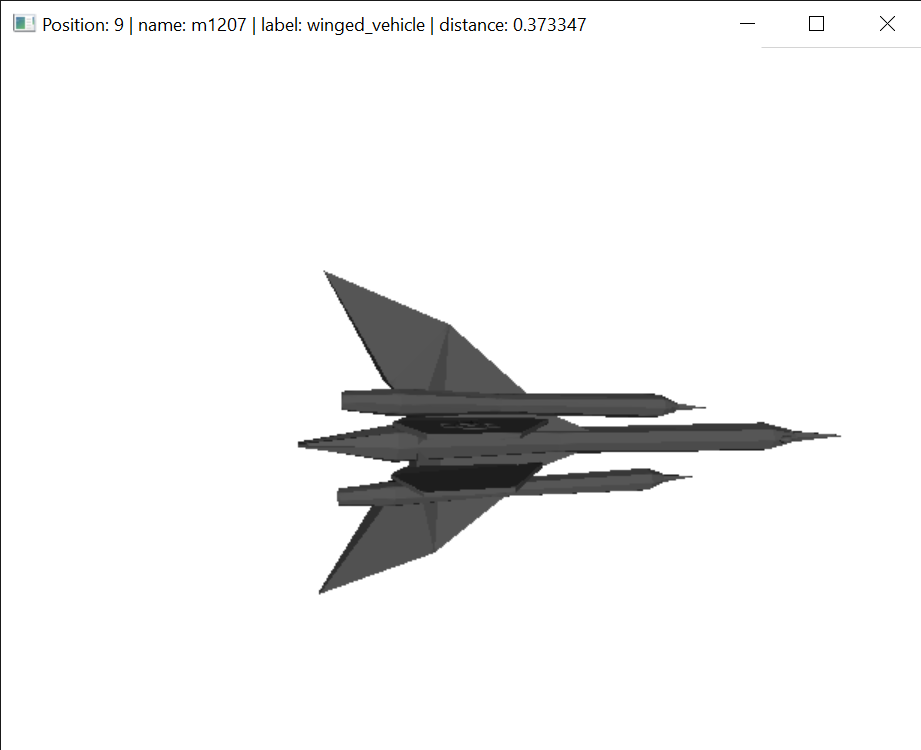
\includegraphics[width=\linewidth]{Pictures/Evaluation/m42/pos9.png}
    \caption*{d=0.37}
  \end{subfigure}

  \centering
  \begin{subfigure}[b]{0.09\linewidth}
    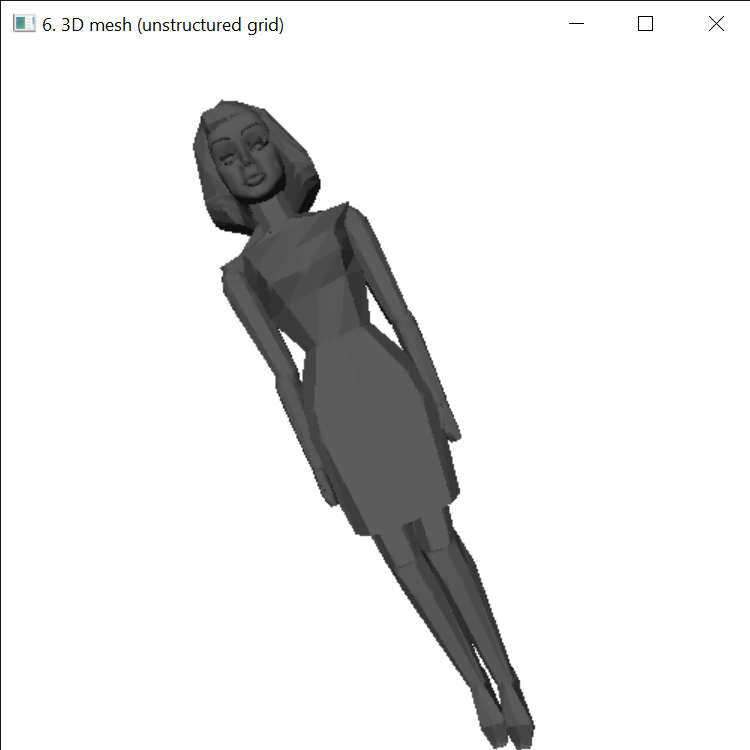
\includegraphics[width=\linewidth]{Pictures/Evaluation/m134/m134.png}
    \caption*{d=0}
  \end{subfigure}
  \begin{subfigure}[b]{0.09\linewidth}
    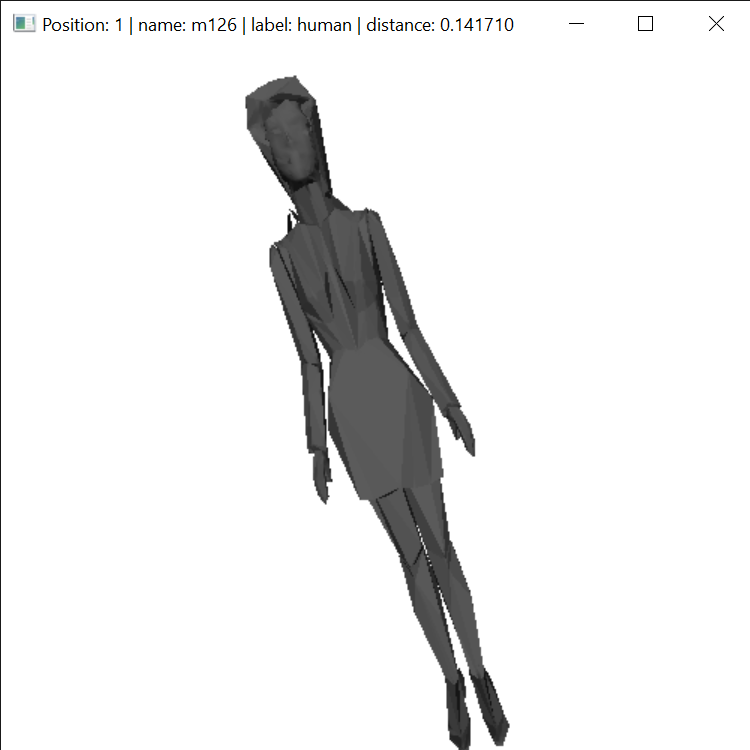
\includegraphics[width=\linewidth]{Pictures/Evaluation/m134/pos1.png}
    \caption*{d=0.14}
  \end{subfigure}
  \begin{subfigure}[b]{0.09\linewidth}
    \includegraphics[width=\linewidth]{Pictures/Evaluation/m134/pos2.png}
    \caption*{d=0.17}
  \end{subfigure}
  \begin{subfigure}[b]{0.09\linewidth}
    \includegraphics[width=\linewidth]{Pictures/Evaluation/m134/pos3.png}
    \caption*{d=0.18}
  \end{subfigure}
  \begin{subfigure}[b]{0.09\linewidth}
    \includegraphics[width=\linewidth]{Pictures/Evaluation/m134/pos4.png}
    \caption*{d=0.19}
  \end{subfigure}
  \begin{subfigure}[b]{0.09\linewidth}
    \includegraphics[width=\linewidth]{Pictures/Evaluation/m134/pos5.png}
    \caption*{d=0.19}
  \end{subfigure}
  \begin{subfigure}[b]{0.09\linewidth}
    \includegraphics[width=\linewidth]{Pictures/Evaluation/m134/pos6.png}
    \caption*{d=0.20}
  \end{subfigure}
  \begin{subfigure}[b]{0.09\linewidth}
    \includegraphics[width=\linewidth]{Pictures/Evaluation/m134/pos7.png}
    \caption*{d=0.20}
  \end{subfigure}
  \begin{subfigure}[b]{0.09\linewidth}
    \includegraphics[width=\linewidth]{Pictures/Evaluation/m134/pos8.png}
    \caption*{d=0.21}
  \end{subfigure}
  \begin{subfigure}[b]{0.09\linewidth}
    \includegraphics[width=\linewidth]{Pictures/Evaluation/m134/pos9.png}
    \caption*{d=0.21}
  \end{subfigure}
  \caption{Query results and their squared distances for models m92, m42, and m134 respectively}
  \label{fig:bunny}
\end{figure}

\section{Conclusion}
This section begins by presenting a summary of our work. Some limitations of our project are then discussed, followed by possible improvements to our implementation and future work.
\subsection{Summary}
This report presented our attempt at a content-based 3D shape retrieval system using scalar features that, given a 3D shape, returns the 10 most similar shapes (excluding itself) from a preprocessed Princeton Shape Benchmark database of 1796 models that are grouped into 53 leaf classes. This search is sped up by the use of a kD-tree and K-nearest neighbors. A visualization of the 65-dimensional feature space is also provided as a 2D plot created using t-SNE. \\
Our system performs much better on some classes, such as humans and winged vehicles, than some other classes, like fireplaces and mailboxes, with an average precision at k=10 of 0.34 and an average MAP of 0.20. We discuss these results in the final section, then provide some query examples.

\subsection{Limitations}

Due to the choice at the start of the project to use 20,000 vertices and the 1800 shape database, database-wide evaluation, recomputing features and reprocessing the database were very slow tasks. In addition, because of the database size, bugs with individual shapes were much harder to detect. For example, some of our shapes started looking like in \textit{Figure 16}.

\begin{figure}[h!]
	\centering
	\begin{subfigure}[b]{0.4\linewidth}
		\includegraphics[width=\linewidth]{Pictures/problem1.png}
		\caption{m1769}
	\end{subfigure}
	\begin{subfigure}[b]{0.4\linewidth}
		\includegraphics[width=\linewidth]{Pictures/problem2.png}
		\caption{m361}
	\end{subfigure}
	\caption{Models with faces missing after surface simplification.}
	\label{fig:problems}
\end{figure}

This turned out to be a problem with our surface simplification algorithm from the PMP library. Some of the shapes were not correctly read by the library, resulting in some of their feature values being affected (i.e. smaller area due to less triangles). Due to the nature of the problem and the time required to solve it, we elected to repair as much of the database as possible and accept that meshes with too many samples would risk to lose some of their faces. This is clearly a priority for any future version of this system.

\pagebreak

\subsection{Improvements \& future work}

There are several parts of our system that could be improved. First and foremost, a different mesh decimation library should be used if we cannot identify what causes the problem with the PMP mesh decimation. \\
Secondly, we could improve the speed of our application by changing the way we compute the diameter. While the method we use right now is much faster than the brute force approach, there are at least two better options to consider. First would be the convex hull approximation which is then used to calculate the diameter much faster, as mentioned in (Xue, J. et al., 2019). Another approach would be to use the technique described by (Har-Peled, S., 2001). \\
Thirdly, we could improve the quality of our matching function by experimenting with different distance functions for our feature vectors. The same can be done for improving the effectiveness of our histogram features by computing their distance a different way, for instance by using the Earth Mover's Distance suggested by (Rubner, Y. et. al., 2000). \\
Lastly, we could optimize matching by changing the weights of features to better reflect the class we are querying for. For example, quadrupeds tend to have a larger surface area, hence increasing this feature's weight would result in better matches. If we could identify the class of the input image, for example by using a classifier trained on the dataset features, we could improve matching by only searching for specific related classes for similar shapes (e.g. when querying for a bird, we would first look through shapes in the bird and winged vehicle class, as they are similar in appearance, even if another shape from an unrelated class would return a smaller distance value). \\
On the visualization side, it would be possible to make a plot that better resembles our system's performance by using a distance matrix as input for the t-SNE algorithm. This was omitted due to time constraints and not being possible in the Python implementation we decided on for ease, but could be much more insightful on how our system actually behaves. In addition to this, it could be possible to perform the entire matching on a simple 2D feature space if our dimensionality reduction resulting plot was reliable enough (with well defined clusters).

\newpage

\section{References}
\paragraph{} Feng, C., Jalba, A. C., \& Telea, A. C. (2016, May). A Descriptor for Voxel Shapes Based on the Skeleton Cut Space. In 3DOR.
\paragraph{} Har-Peled, S. (2001, June). A practical approach for computing the diameter of a point set. In Proceedings of the seventeenth annual symposium on Computational geometry (pp. 177-186). ACM.
\paragraph{} Körtgen, M., Park, G. J., Novotni, M., \& Klein, R. (2003, April). 3D shape matching with 3D shape contexts. In The 7th central European seminar on computer graphics (Vol. 3, pp. 5-17). Budmerice.
\paragraph{} Maaten, L. V. D., \& Hinton, G. (2008). Visualizing data using t-SNE. Journal of machine learning research, 9(Nov), 2579-2605.
\paragraph{} Rubner, Y., Tomasi, C., \& Guibas, L. J. (2000). The earth mover's distance as a metric for image retrieval. International journal of computer vision, 40(2), 99-121.
\paragraph{} Shilane, P., Min, P., Kazhdan, M., \& Funkhouser, T. (2004, June). The princeton shape benchmark. In Proceedings Shape Modeling Applications, 2004. (pp. 167-178). IEEE.
\paragraph{} Song, J. (2017). Indexing Techniques for Multimedia Data Retrieval. Encyclopedia of Database Systems, 1-6.
\paragraph{} Tangelder, J. W. H., \& Veltkamp, R. C. (2007). A survey of content based 3D shape retrieval methods. Multimedia Tools and Applications, 39(3), 441–471.
\paragraph{} Vranic, D. V., \& Saupe, D. (2004). 3D model retrieval (Doctoral dissertation, University of Leipzig).
\paragraph{} Xue, J., Li, Y., \& Janardan, R. (2019). On the expected diameter, width, and complexity of a stochastic convex hull. Computational Geometry, 82, 16-31.
\end{document}
